% !TEX TS-program = pdflatex
% !TEX encoding = UTF-8 Unicode

\documentclass{beamer}

\mode<presentation>
{
  \usetheme{Warsaw}
  % or ...

  \setbeamercovered{transparent}
  % or whatever (possibly just delete it)
}


\usepackage[english]{babel}
% or whatever
\usepackage{graphicx}

\usepackage[utf8]{inputenc}
% or whatever

\usepackage{times}
\usepackage[T1]{fontenc}
% Or whatever. Note that the encoding and the font should match. If T1
% does not look nice, try deleting the line with the fontenc.


\title[Short Paper Title] % (optional, use only with long paper titles)
{Critical states of slow pattern in neuronal networks}

%\subtitle
%{Include Only If Paper Has a Subtitle}

\author[Author, Another] % (optional, use only with lots of authors)
{Longbin Zeng\inst{1} \and S.~Another\inst{2}}
% - Give the names in the same order as the appear in the paper.
% - Use the \inst{?} command only if the authors have different
%   affiliation.

\institute[Universities of Somewhere and Elsewhere] % (optional, but mostly needed)
{
  \inst{1}%
  Department of Computer Science\\
  University of Somewhere
  \and
  \inst{2}%
  Department of Theoretical Philosophy\\
  University of Elsewhere}
% - Use the \inst command only if there are several affiliations.
% - Keep it simple, no one is interested in your street address.

\date[CFP 2003] % (optional, should be abbreviation of conference name)
{Conference on Fabulous Presentations, 2003}
% - Either use conference name or its abbreviation.
% - Not really informative to the audience, more for people (including
%   yourself) who are reading the slides online

\subject{Theoretical Computer Science}
% This is only inserted into the PDF information catalog. Can be left
% out. 



% If you have a file called "university-logo-filename.xxx", where xxx
% is a graphic format that can be processed by latex or pdflatex,
% resp., then you can add a logo as follows:

% \pgfdeclareimage[height=0.5cm]{university-logo}{university-logo-filename}
% \logo{\pgfuseimage{university-logo}}



% Delete this, if you do not want the table of contents to pop up at
% the beginning of each subsection:
\AtBeginSubsection[]
{
  \begin{frame}<beamer>{Outline}
    \tableofcontents[currentsection,currentsubsection]
  \end{frame}
}


% If you wish to uncover everything in a step-wise fashion, uncomment
% the following command: 

%\beamerdefaultoverlayspecification{<+->}


\begin{document}

\begin{frame}
  \titlepage
\end{frame}

\begin{frame}{Outline}
  \tableofcontents
  % You might wish to add the option [pausesections]
\end{frame}


% Structuring a talk is a difficult task and the following structure
% may not be suitable. Here are some rules that apply for this
% solution: 

% - Exactly two or three sections (other than the summary).
% - At *most* three subsections per section.
% - Talk about 30s to 2min per frame. So there should be between about
%   15 and 30 frames, all told.

% - A conference audience is likely to know very little of what you
%   are going to talk about. So *simplify*!
% - In a 20min talk, getting the main ideas across is hard
%   enough. Leave out details, even if it means being less precise than
%   you think necessary.
% - If you omit details that are vital to the proof/implementation,
%   just say so once. Everybody will be happy with that.

\section{Motivation}

\subsection{The Basic Problem That We Studied}

\begin{frame}{Network Dynamics}  % {Subtitles are optional.}
  % - A title should summarize the slide in an understandable fashion
  %   for anyone how does not follow everything on the slide itself.

  \begin{itemize}
  \item
    Network response correspond to specific neuronal parameter, including fire rate, degree of irregularity, spatiotemporal patterns in neuronal spike trains and neuronal critical dynamics.
  \item
	Explor the influence of simulation size of neuronal network as well as the community stuctural network. 2000, 5000, 10000, ..., 100 million. 
  \item 
  Synapase density and input heterogeneity.(to be confirmed)
  \end{itemize}
\end{frame}



\begin{frame}{Theoretical explanation}

  Mainly three aspects\ldots
  \begin{itemize}
  \item Explain the mechanism underly the trainsition dynamics.
    \begin{itemize}
    \item 
    input current variablity analysis.
    \item
      Mean-filed equation and hopf bifuraction
    \item    
      The real part of fixed point is decreasing.
    \end{itemize}
  \item
   fit the network response with a simple f unction.
  \end{itemize}
\end{frame}


\subsection{Previous Work}

\begin{frame}{Make Titles Informative.}
\end{frame}

\begin{frame}{Make Titles Informative.}
\end{frame}



\section{Our Results/Contribution}

\subsection{Main Results}
\begin{frame}{signle neuron dynamics}
	Orinignal model
	\begin{equation*}
		C_{j} \dot{V_{j}}  = - \sum_{A=L, E, I}g_{A}^{j}(V_{j} - E_{A}),
	\end{equation*}
	where $\dfrac{g_{E, I}^{j}}{g_{L}^{j}}=\tau_{j}\sum_{m} \sum_{k|t_{m}^{k}<t}\int_{-\infty}^{t}dt^{\prime}a_{\tau_{decay}}\left(t - t^{\prime}\right) \delta(t^{\prime}-t_{m}^{k})$, usually, $a_{\tau_{decay}}(t)=e^{-t / \tau_{decay}} / \tau_{decay}$, but here we use the limit that $\tau_{decay} \rightarrow 0$.
\end{frame}

\begin{frame}{signle neuron dynamics}
	\begin{itemize}
		\item excitatory and inhibitory currents must be fine-tuned to produce an average input below threshold. Specifically, if K and J represent the average number of input connections per neuron and synaptic efficacy, respectively, the difference between excitatory and inhibitory presynaptic inputs must be of the order of $1/KJ$.
		\item input fluctuations should be large enough to drive firing.
	\end{itemize}
\end{frame}

\begin{frame}{signle neuron dynamics}
	We can use the diffusion approximation and approximate the conductances as
	\begin{equation}
		\begin{aligned}
			&\frac{g_{E}}{g_{L}}=a \tau_{L}\left[K r_{E}+\sqrt{K r_{E}} \zeta_{E}\right], \\
			&\frac{g_{I}}{g_{L}}=a g \tau_{L}\left[\gamma K r_{I}+\sqrt{\gamma K r_{I}} \zeta_{I}\right]
		\end{aligned}
	\end{equation}
\end{frame}

\begin{frame}{signle neuron dynamics}
	Using the diffusion approximation, OU process, the CV equation can be reduced to
	\begin{equation}
		\tau \frac{d V}{d t}=-V+\mu+\sigma(V) \sqrt{\tau} \zeta
	\end{equation}
	where
	\begin{equation}
		\begin{aligned}
			\tau^{-1} &=\tau_{L}^{-1}+a K\left(r_{E}+r_{I} g \gamma\right) \\
			\mu &=\tau\left\{E_{L} / \tau_{L}+a K\left[r_{E} E_{E}+r_{I} g \gamma E_{I}\right]\right\} \\
			\sigma^{2}(V) &=a^{2} K \tau\left[r_{E}\left(V-E_{E}\right)^{2}+g^{2} \gamma r_{I}\left(V-E_{I}\right)^{2}\right]
		\end{aligned}
	\end{equation}
\end{frame}
\begin{frame}
	under the assumption that $Ka >> 1$, we have
	\begin{equation}\label{scaling_function}
		\tau \sim \frac{\tau_{0}^{\text {cond }}}{K a}, \quad \mu \sim \mu_{0}^{\text {cond }}, \quad \sigma \sim \sqrt{a} \sigma_{0}^{\text {cond }}
	\end{equation}
	we can conclude that:
	\begin{enumerate}
		\item $\mu$ is indenpendent of coupling strength, i.e, the synaptic efficacy $a$ and degree $k$.
		\item Increasing $a$ modifies the drift force and the input noise, which increase proportionally to $a$ and $\sqrt{a}$
		\item incresing $k$ increases the drift force as $ka$
	\end{enumerate}
	In this case, $ka >> 1$, we called it strong coupling. However, if such assumpaiton not holds (weak coupling), the scaling function \eqref{scaling_function} is not ture.
\end{frame}

\begin{frame}{Biological plausible neuronal network}
	Consider a balanced E-I network with $ N $ neurons, in which $ 80\% $  are excitatory neurons and the others inhibitory ones. Each neuron is equipped with a biological plausible neuronal model, leaky integrate and fire model, 
	\begin{equation*}
		C \dfrac{dV}{dt} = -g_{l}(V - V_{l}) + I_{syn} + I_{ext},
	\end{equation*}
	and the conductance-based synaptical filter
	\begin{equation*}
		\begin{aligned}
			&I_{syn}(t) = \sum_{u} g_{u} S_{u}(t)(V_{rev, u} - V)\\
			&S_{i, u}(t) = \dfrac{1}{\tau_{u}}e^{-t /\ \tau_{u}} \ast \sum_{n, j \in \partial ^{i}} w_{j} \delta \left(t - t_{j}^{n}\right)\\
			&u=\{AMPA, NMDA, GABA_{A}, GABA_{B}\}.
		\end{aligned}
	\end{equation*}
\end{frame}



\begin{frame}{Balance condition}
	Under the given network conditions and default neuron parameters, we need to seek for a group of appropriate parameters ($ g_{u} $) to make the network self-sustaining in a stable firing state.
	
	\par 
	we can roughly estimate a gruop of parameter by adopting the first order diffusion approximation.
	\begin{equation*}
		\dfrac{V_{th} - V_{reset}}{\sum_{u} \langle g_{u}S_{u}(V_u - V) \rangle - \langle g_{l}(V - V_{l})\rangle} = \dfrac{1 }{r_{\text{equilibrium}}},
	\end{equation*}	
	and then we can dervie that
	\begin{equation}
		\label{eq:param_restriction}
		\left\{
		\begin{aligned}
			&1 g_{AMPA} + 5 g_{NMDA} = 0.022 \\
			&1 g_{GABA_{A}} + 18 g_{GABA_{B}} = 0.5\\
		\end{aligned}
		\right .
	\end{equation}
	\par 
	
\end{frame}

\begin{frame}{Default Paramters}
	\begin{table}
		\centering
		\begin{tabular}{lll}
			Symbol & Description & Value\\
			\hline
			$N$ & Total number of neurons & $2000$\\
			$N_{E}$ & Total number of excitatory neurons & $1600$ \\
			$N_{I}$ & Total number of inhibitory neurons & $400$ \\
			$K_{in}$ &  Mean of in-degrees & $100$ \\
			$\tau_{ref}$ & Refractory period & $5ms$ \\
			$tau_{u}$ & decay time of receptors & $(8, 40, 10, 50)$ \\
			$V_{rev, u}$ & reverse voltage & $(0, 0, -70, -100))$ \\
		\end{tabular}
		\caption{Default values of model parameters used in numerical simulations}
		\label{tab:model_tabel}
	\end{table}
\end{frame}

\begin{frame}{Rich dynamics in parameter submainfold}
	\begin{columns}
		\column{0.49\linewidth}
		We find rich dynamics in this small balanced E-I network.
		\begin{itemize}
			\item Obvious transition in the fire rate.
			\item CV is larger than 1, and multi stratification.
			\item Coherence coefficient reflects the spike coherence.
			\item Critical dynamics occurs in the stratification line paramete space.
		\end{itemize}
		\column{0.55\linewidth}
		\begin{figure}[htbp]
			\centering
			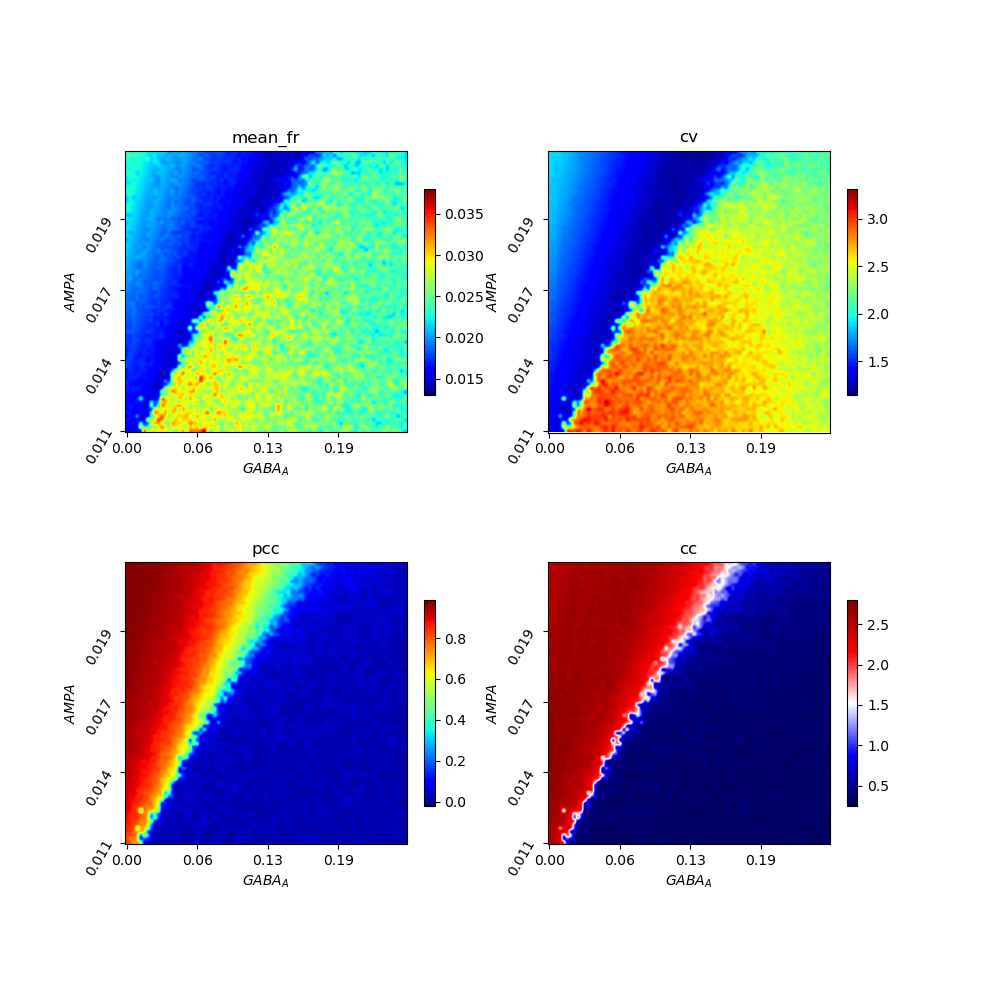
\includegraphics[scale=0.25]{fig/phase_plot}
		\end{figure}
	\end{columns}
\end{frame}

\begin{frame}{avalanches pehenomena}
	Mainly due to E-I delay feedback$\ldots$
	\begin{figure}[htbp]
		\centering
		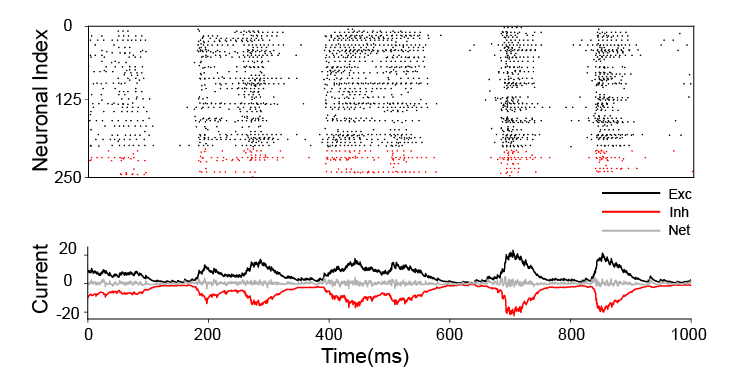
\includegraphics[width=0.9\linewidth]{fig/raster}
		\caption{raster plot of slow dynamics}
		\label{raster plot}
	\end{figure}
\end{frame}
	
\begin{frame}{avalanches pehenomena}
	\begin{figure}[htbp]
		\centering
		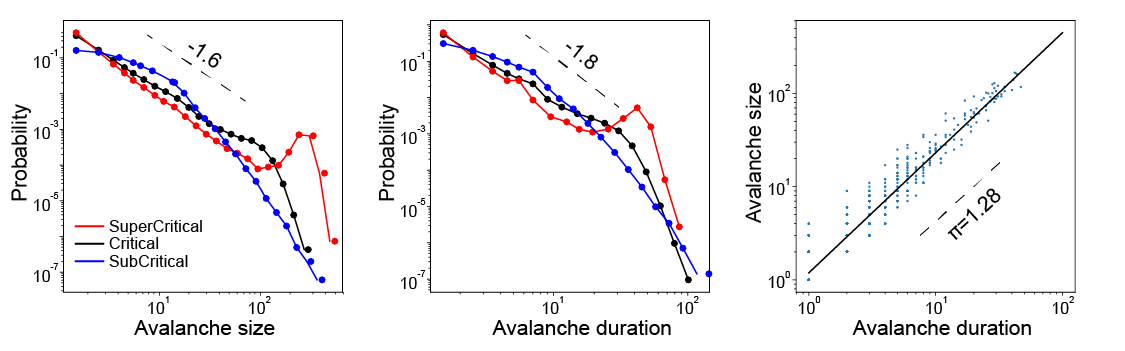
\includegraphics[width=0.9\linewidth]{fig/avalanches_distribution}
		\caption{avalanches pehenomena}
	\end{figure}
	The slope of best fit powerlaw distribution for avalanche size is $ -1.6 $ and avalanche duration is $ -1.8 $
\end{frame}

\begin{frame}{Characteristic in boundary line}
	if we dive into the characteristices of the network on the boundary line space
	\begin{figure}[htbp]
		\centering
		\begin{minipage}{0.48\linewidth}
			\centering
			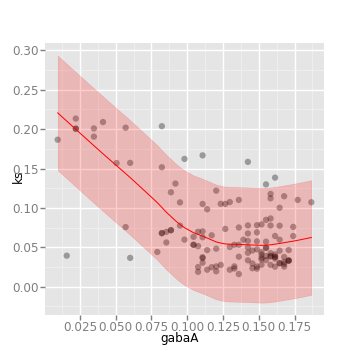
\includegraphics[width=0.85\linewidth]{fig/along_critical_ks}
			\caption{ks distance}
		\end{minipage}
		%\qquad
		\begin{minipage}{0.48\linewidth}
			\centering
			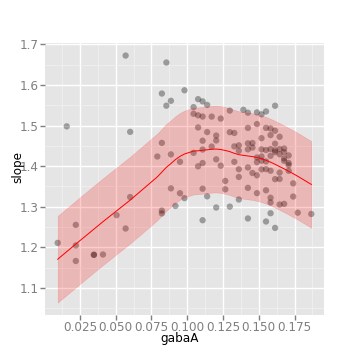
\includegraphics[width=0.85\linewidth]{fig/along_critical_slope}
			\caption{slope}
		\end{minipage}
	\end{figure}
\end{frame}

\begin{frame}{robust on size}
	\begin{columns}
		\column{0.49\linewidth}
		The corresponding relationship between \textit{coherence coefficient} and \textit{ks distance} is shown in the figure below
		\centering
		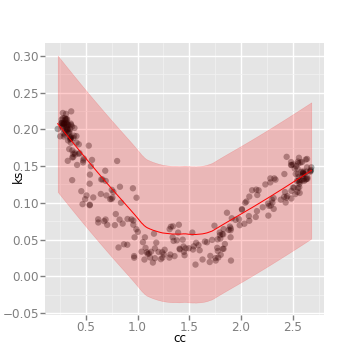
\includegraphics[width=0.85\linewidth]{fig/cc_vc_ks}
		\column{0.55\linewidth}
		\begin{figure}[htbp]
			\centering
			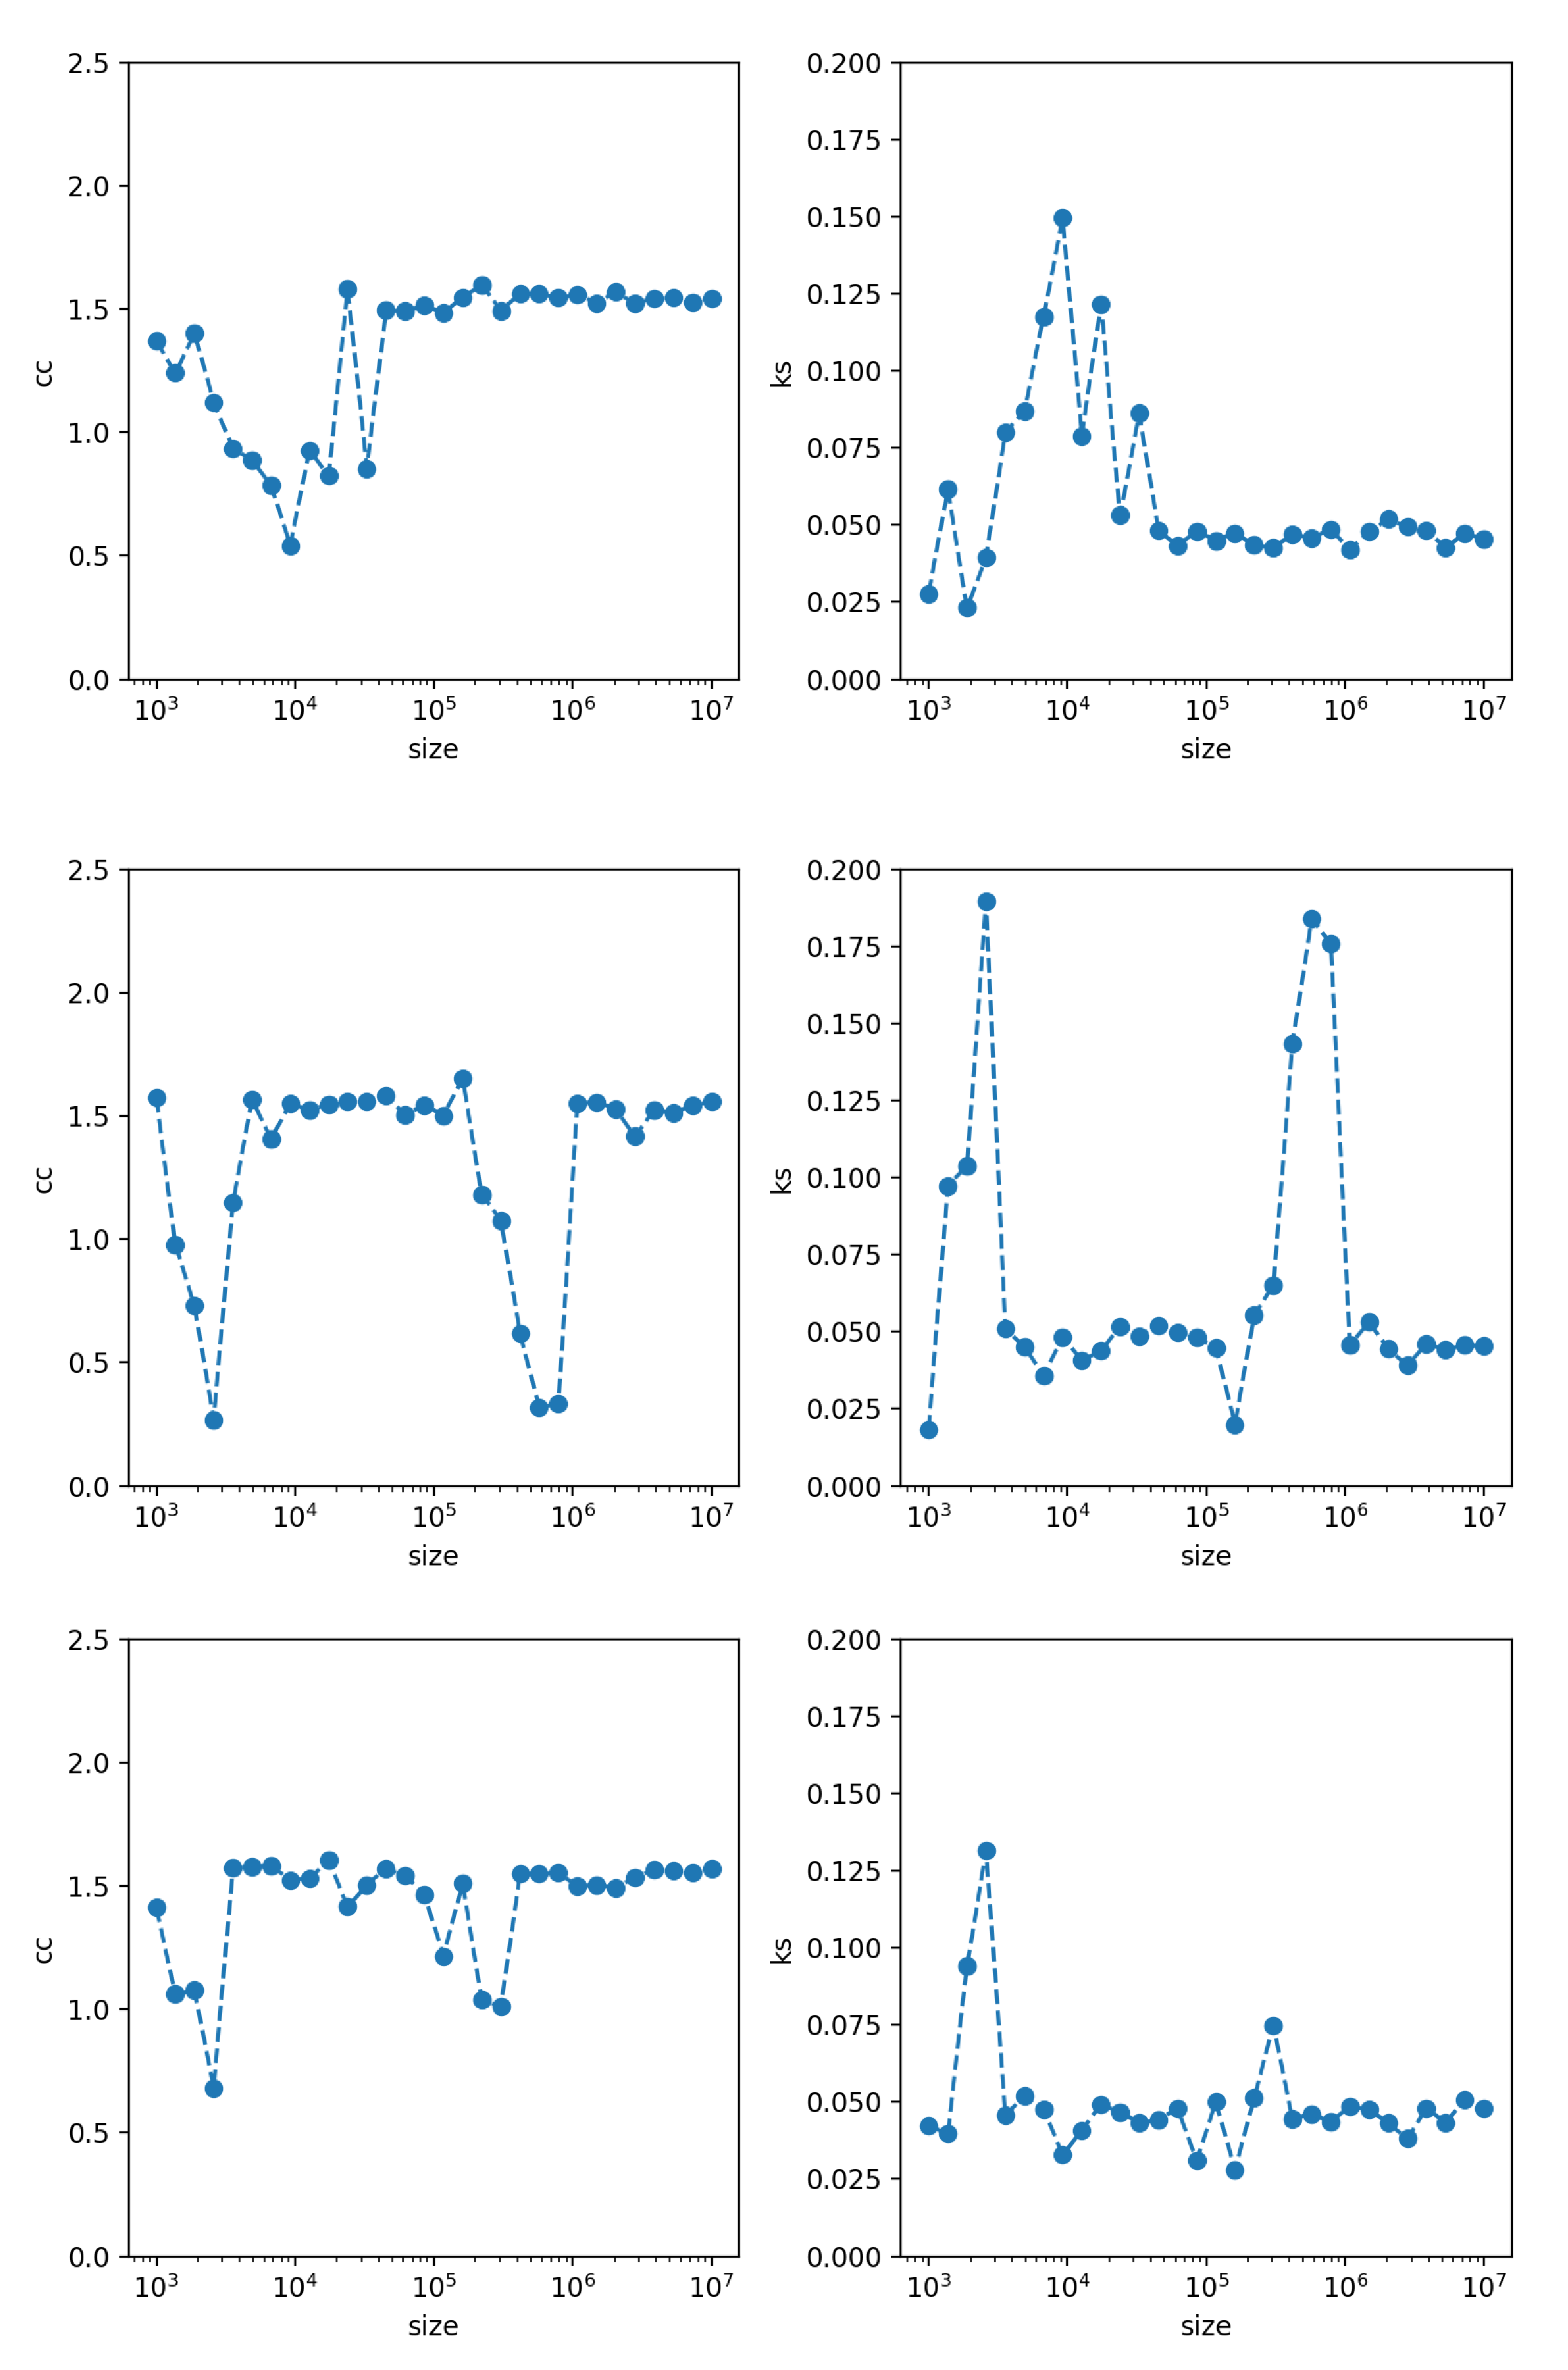
\includegraphics[scale=0.2]{fig/size_influence_total}
		\end{figure}
	\end{columns}
\end{frame}

\begin{frame}{degree inluence}
	we perform experiments and summarize the main findings based on shifted exponential in- degree distributions.
	\centering
	\begin{figure}[htbp]
	\centering
	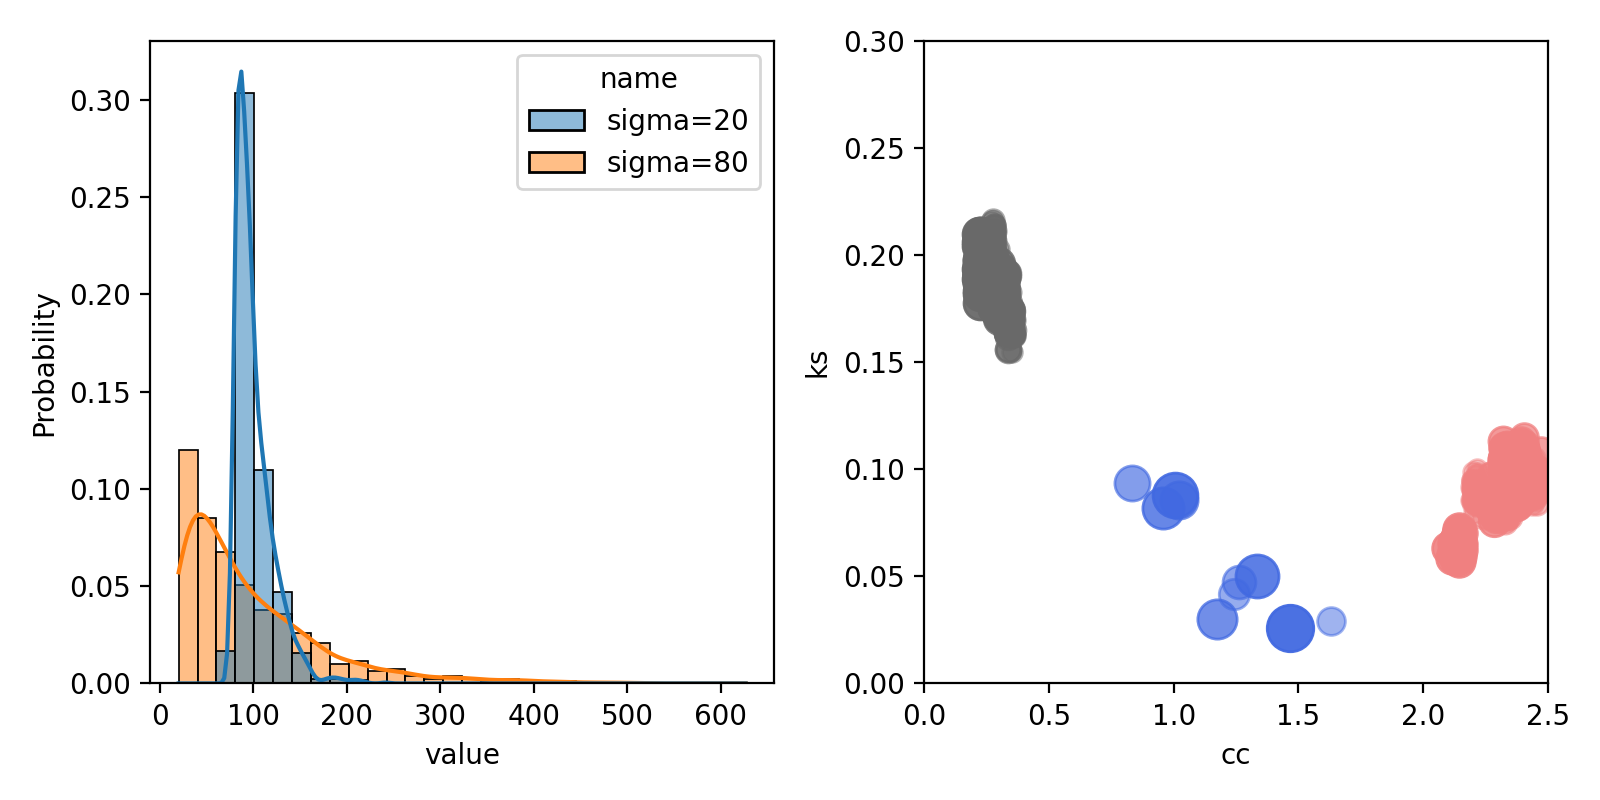
\includegraphics[width=0.85\linewidth]{fig/degree_influence}
	\caption{degree influence}
	\end{figure}
\end{frame}

\begin{frame}{parameter heterogeneity}
	\begin{itemize}
		\item the raidus is from 1 to 15
		\item along the boundary line
	\end{itemize}
	\centering
	\begin{figure}[htbp]
		\centering
		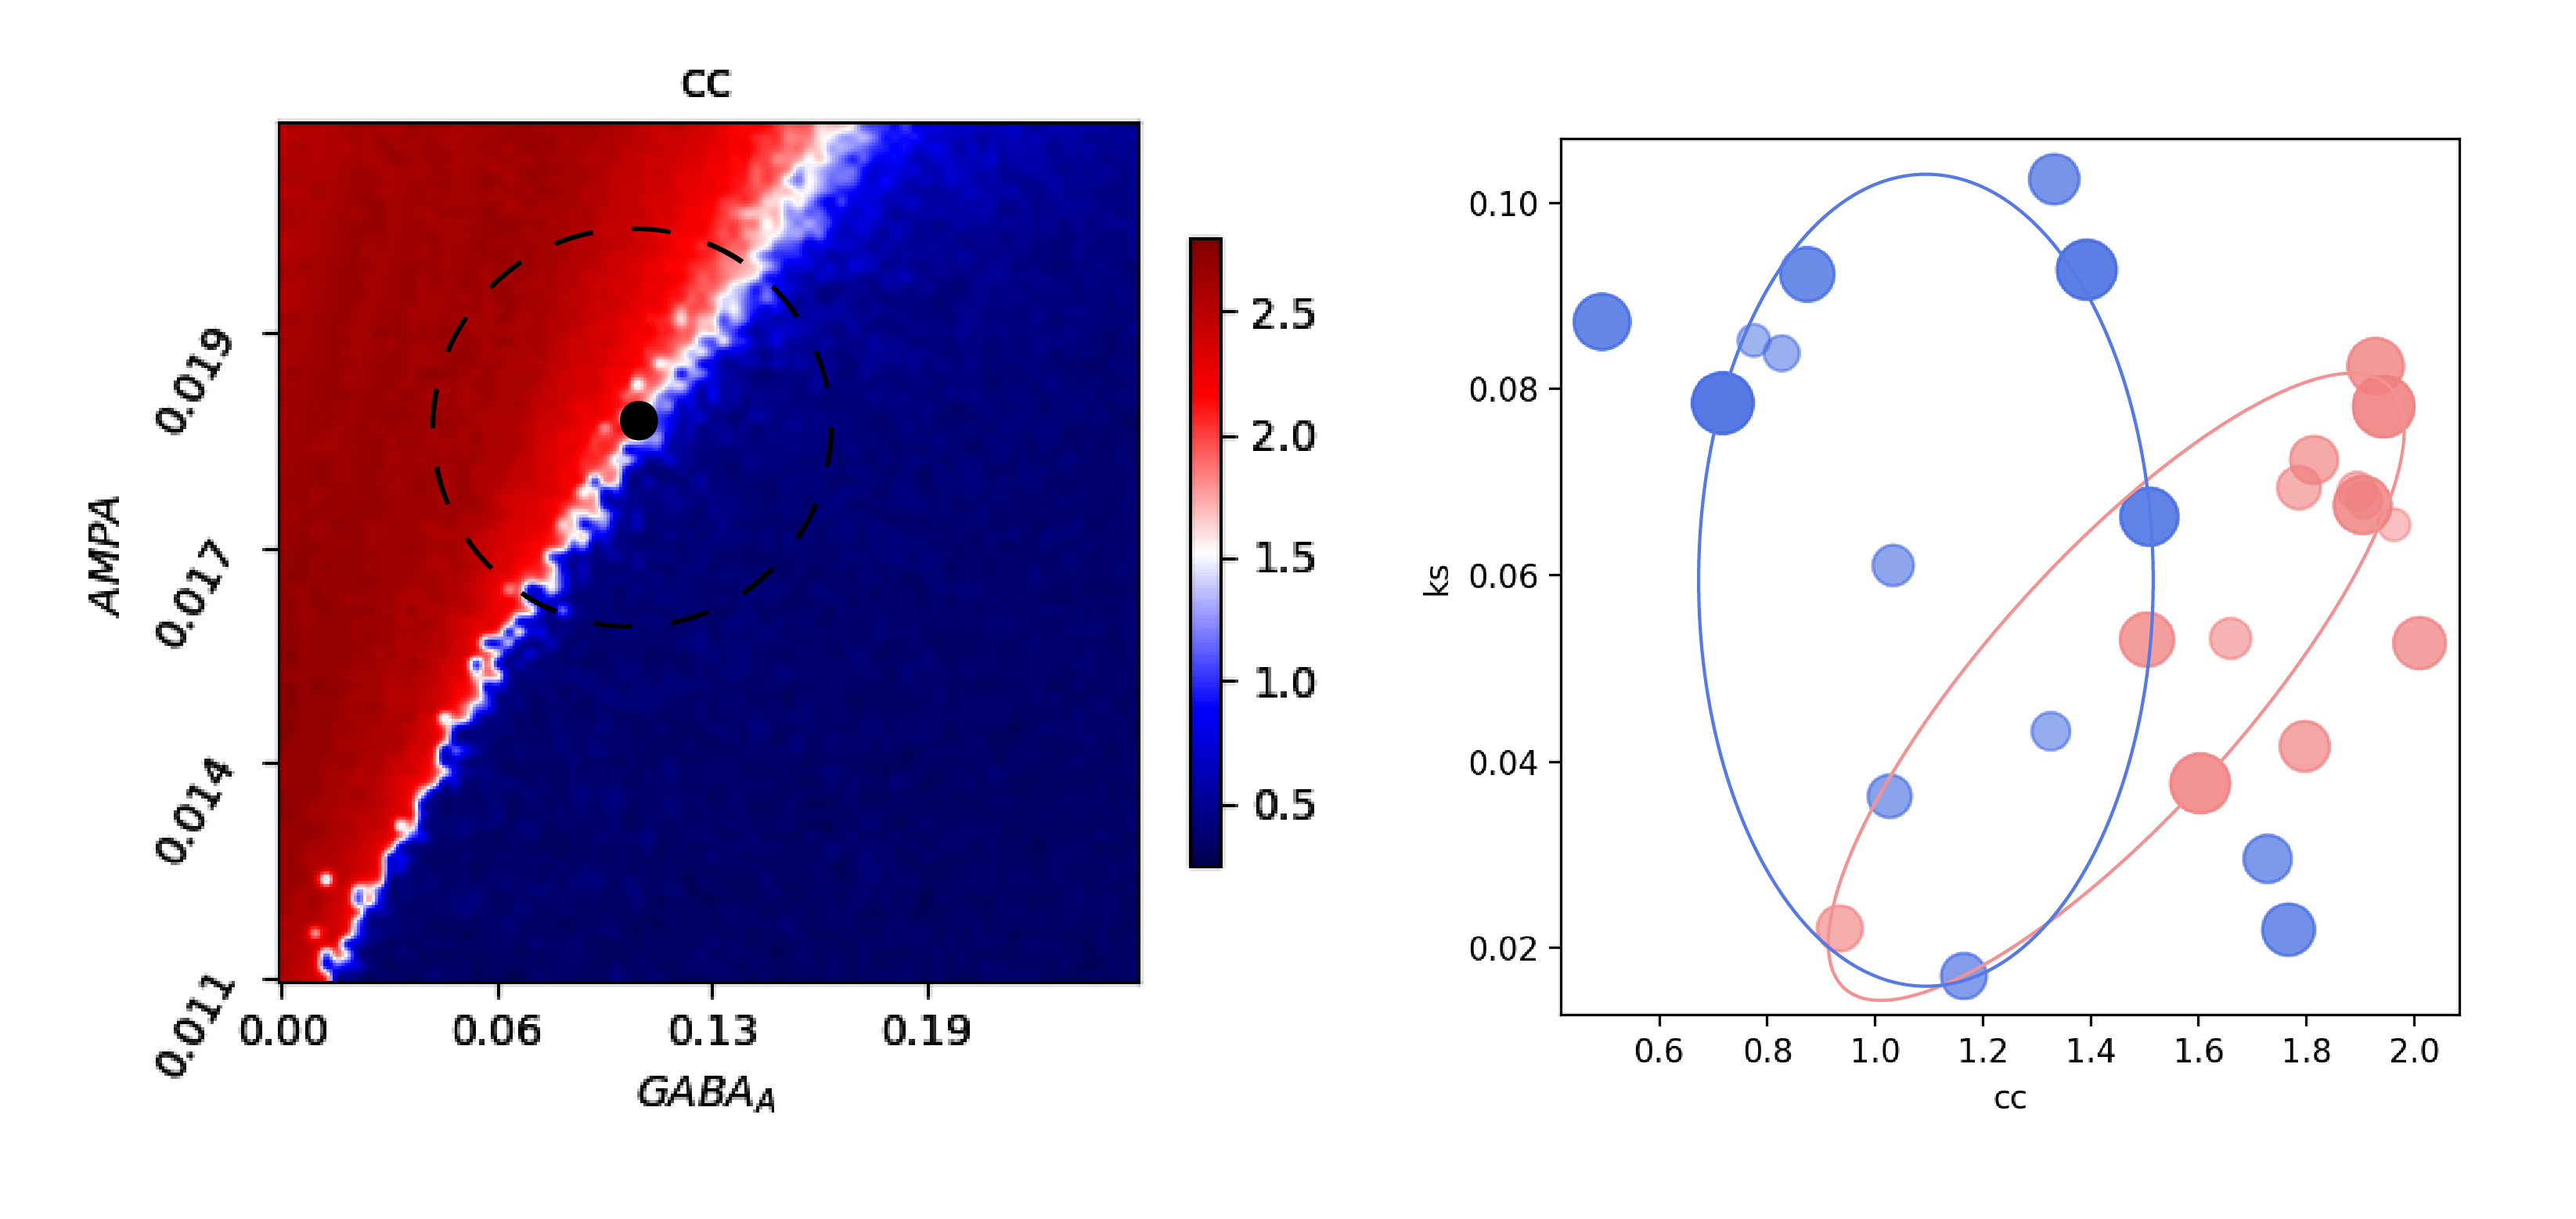
\includegraphics[width=0.8\linewidth]{fig/reparameter_all}
		\caption{parameter heterogeneity} 
	\end{figure}
\end{frame}

\begin{frame}{Criticality in large-scale network}
	Fit to function $ s\cdot tanh(ax+by+c) + t $
	\begin{itemize}
		\item in the small blcok, slop is $1.6$
		\item in the large-scale block, slop is $1.6$
	\end{itemize}
\begin{figure}[htbp]
	\centering
	\begin{minipage}{0.49\linewidth}
		\centering
		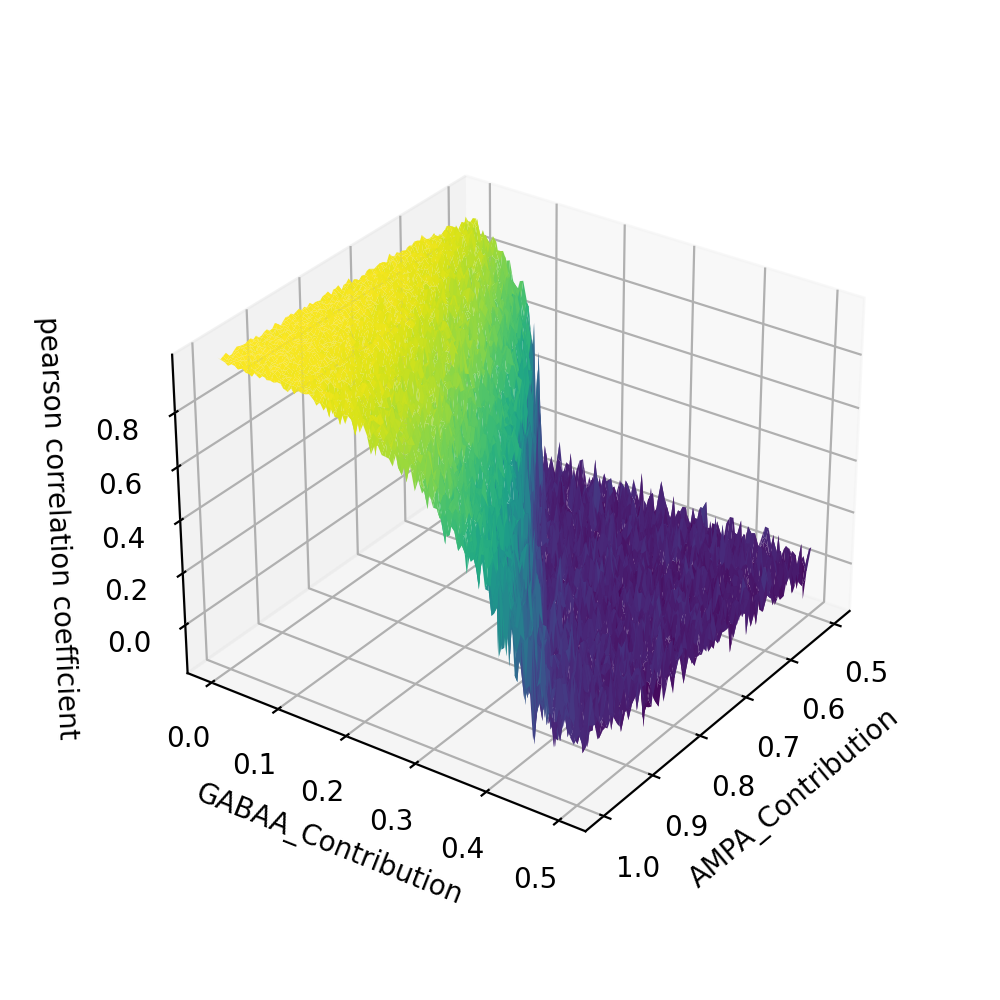
\includegraphics[width=0.85\linewidth]{fig/small_block_dense_grid_pcc}
		\caption{size=2k}
		\label{small_block}
	\end{minipage}
	%\qquad
	\begin{minipage}{0.49\linewidth}
		\centering
		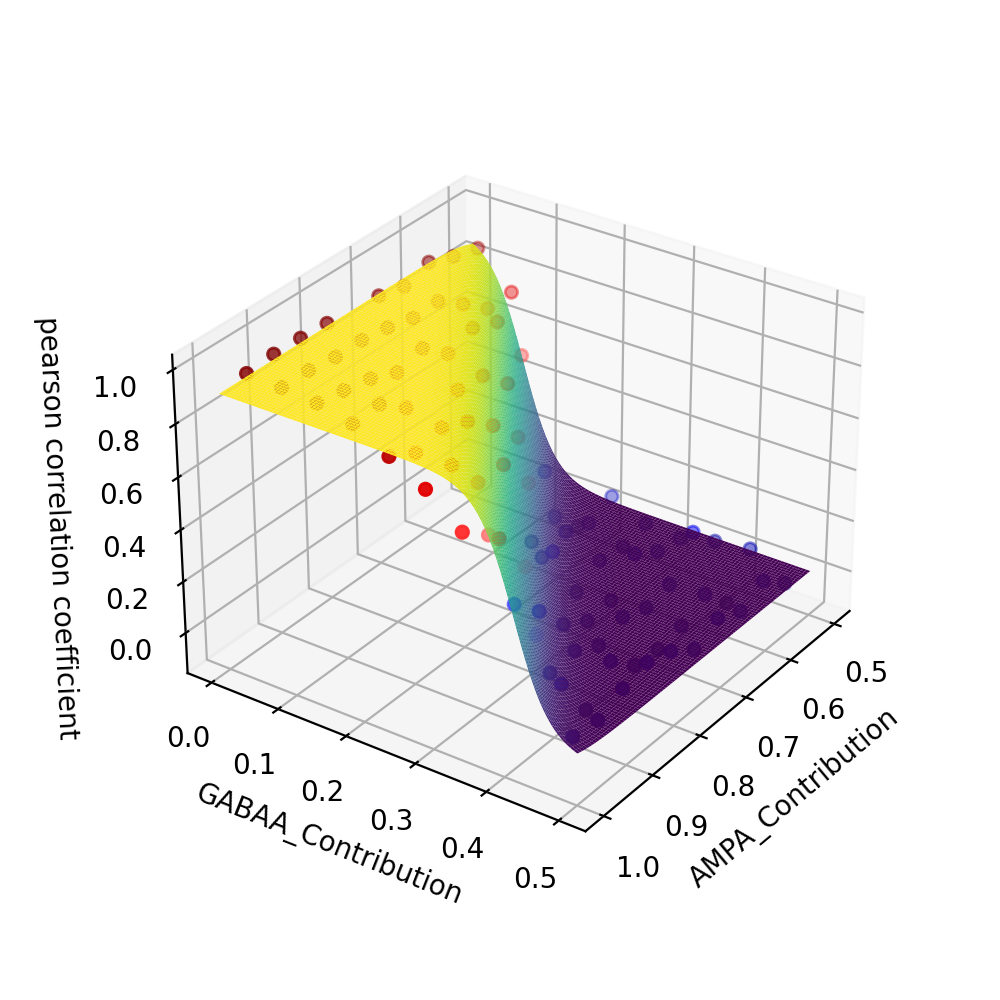
\includegraphics[width=0.85\linewidth]{fig/100m_block_sparse_point_pcc}
		\caption{size=100m}
		\label{big_block}
	\end{minipage}
\end{figure}
\end{frame}



\begin{frame}{Criticality in large-scale network}
		\begin{figure}[htbp]
		\centering
		\begin{minipage}{0.49\linewidth}
			\centering
			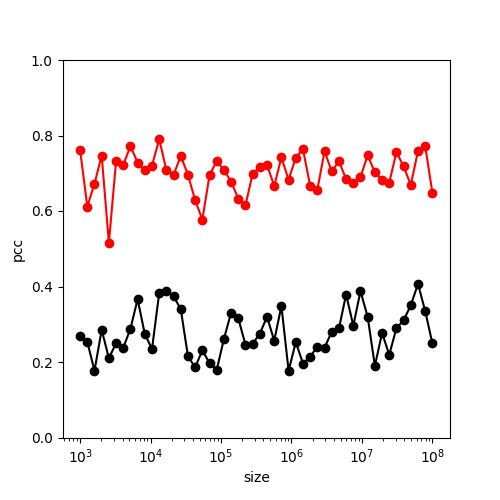
\includegraphics[width=0.9\linewidth]{fig/size_influence}
			\caption{pcc with respect to different sizes}
		\end{minipage}
		%\qquad
		\begin{minipage}{0.49\linewidth}
			\centering
			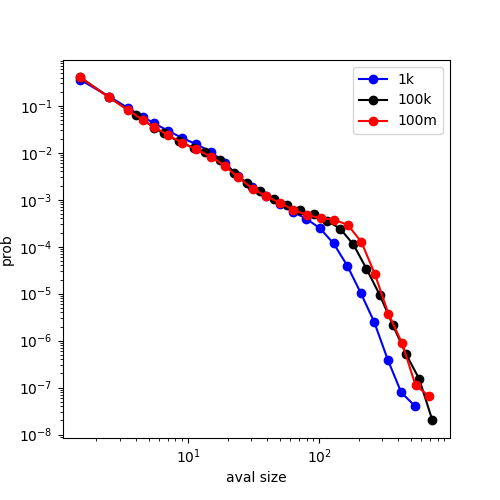
\includegraphics[width=0.9\linewidth]{fig/multi_size_avalanches}
			\caption{avalanches distribution}
		\end{minipage}
	\end{figure}
\end{frame}

\begin{frame}{Criticality in large-scale network}
	Some simulation case from a fixed parameter of critical space.
	\begin{itemize}
		\item The avalanche size increases with the size of the simulation.
	\end{itemize}
	\begin{figure}[htbp]
		\centering
		\begin{minipage}{0.49\linewidth}
			\centering
			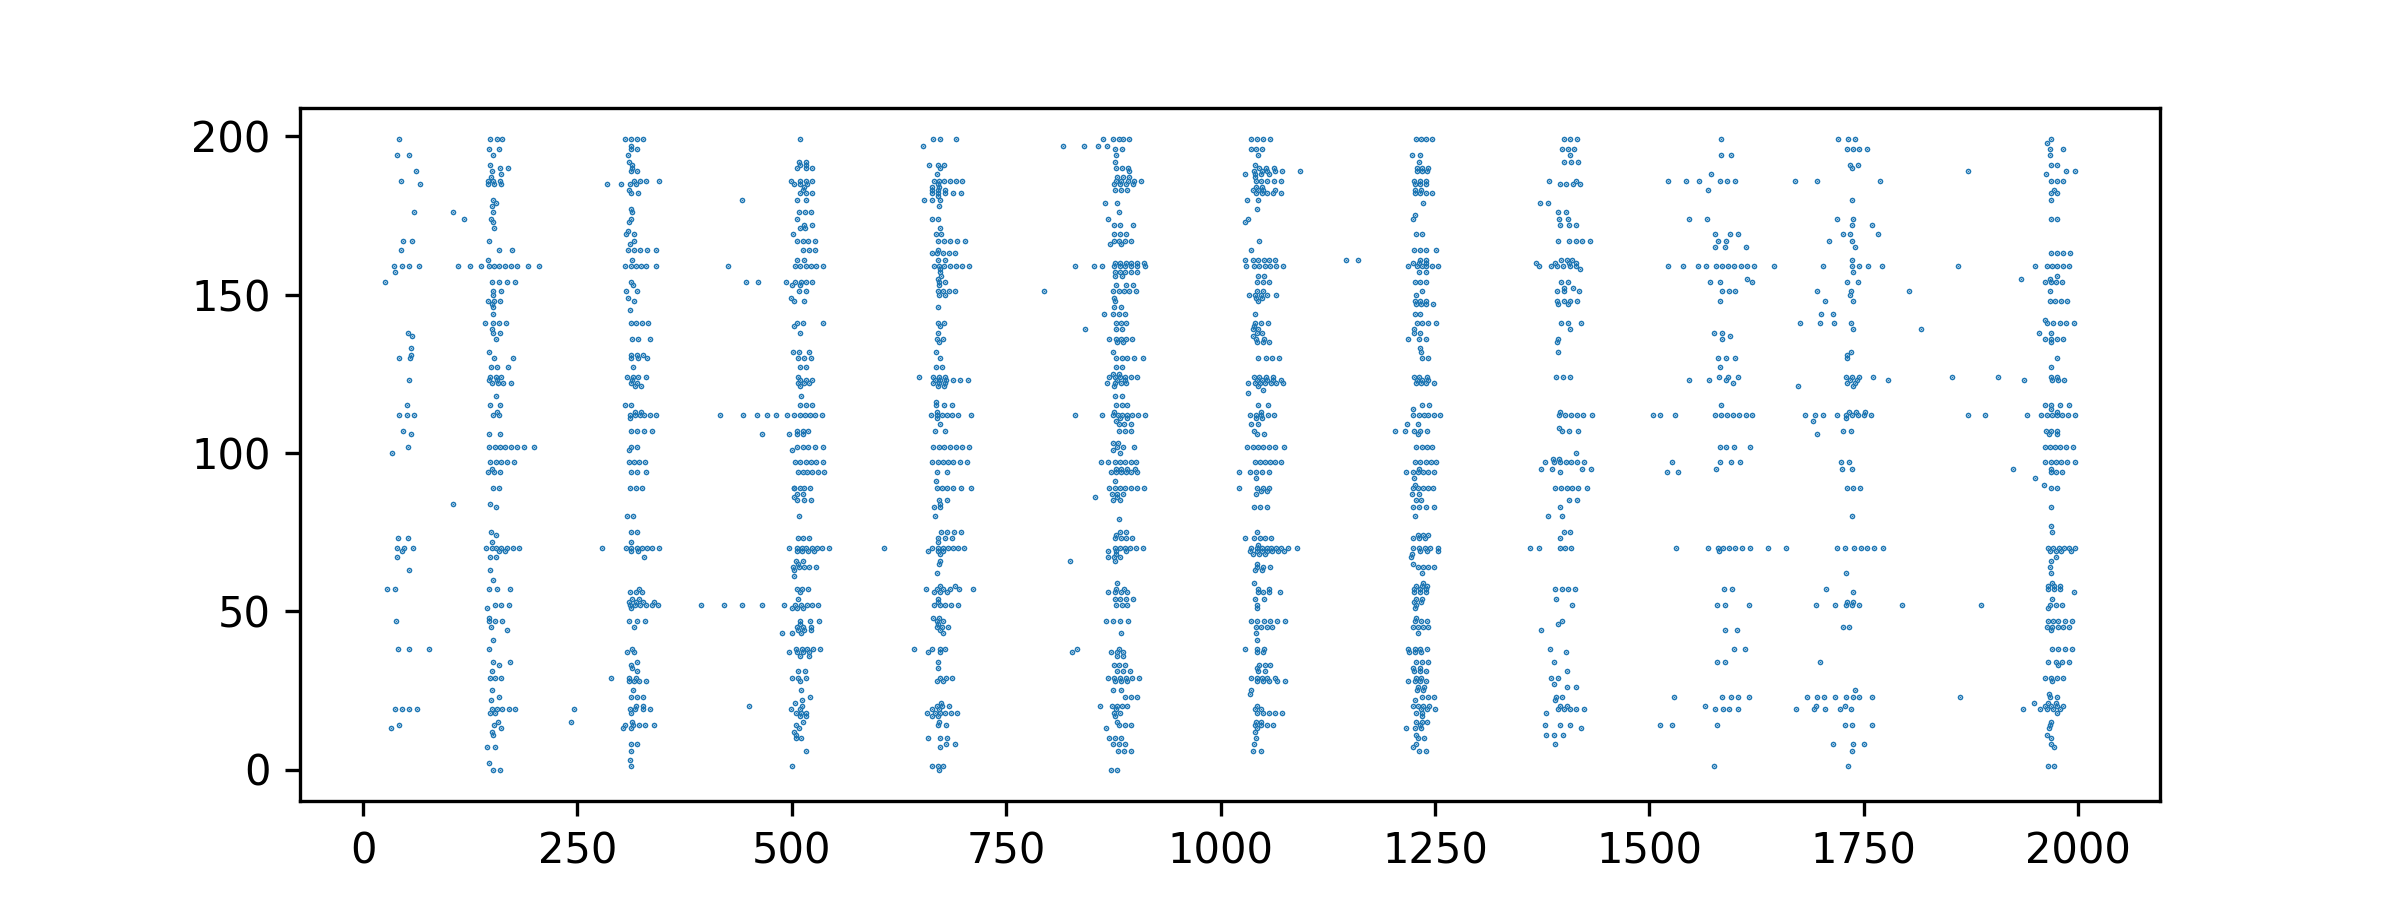
\includegraphics[width=0.9\linewidth]{fig/from_critical_size_10k}
			\caption{size=10k}
			\label{small_block}
		\end{minipage}
		%\qquad
		\begin{minipage}{0.49\linewidth}
			\centering
			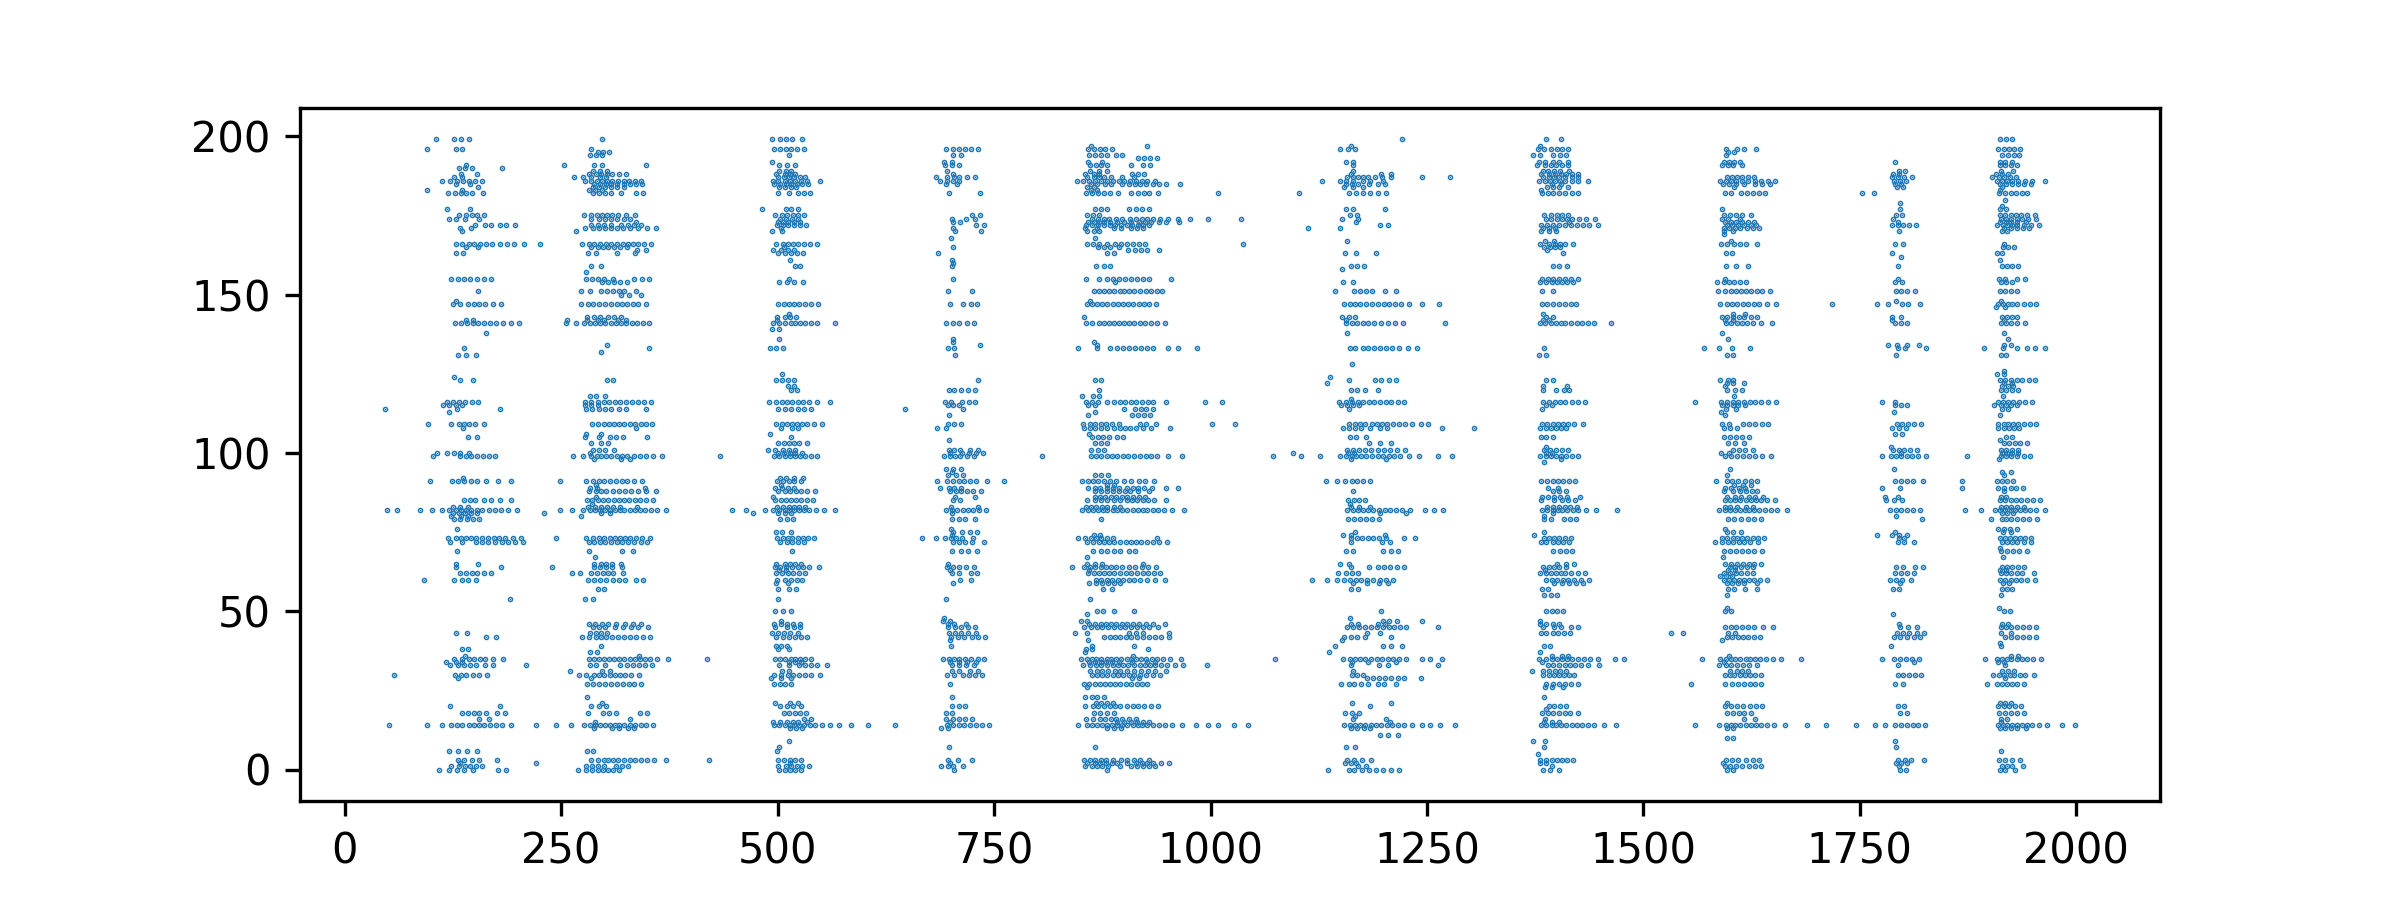
\includegraphics[width=0.9\linewidth]{fig/from_critical_size_100m}
			\caption{size=100m}
			\label{big_block}
		\end{minipage}
	\end{figure}
\end{frame}

\begin{frame}{Dependence on connection density}
	grid search on network of 2000 neurons with 300 in-connections. x and y range is $ [0, 1] $, each $ 50 $ points.
	\begin{figure}[htbp]
		\centering
		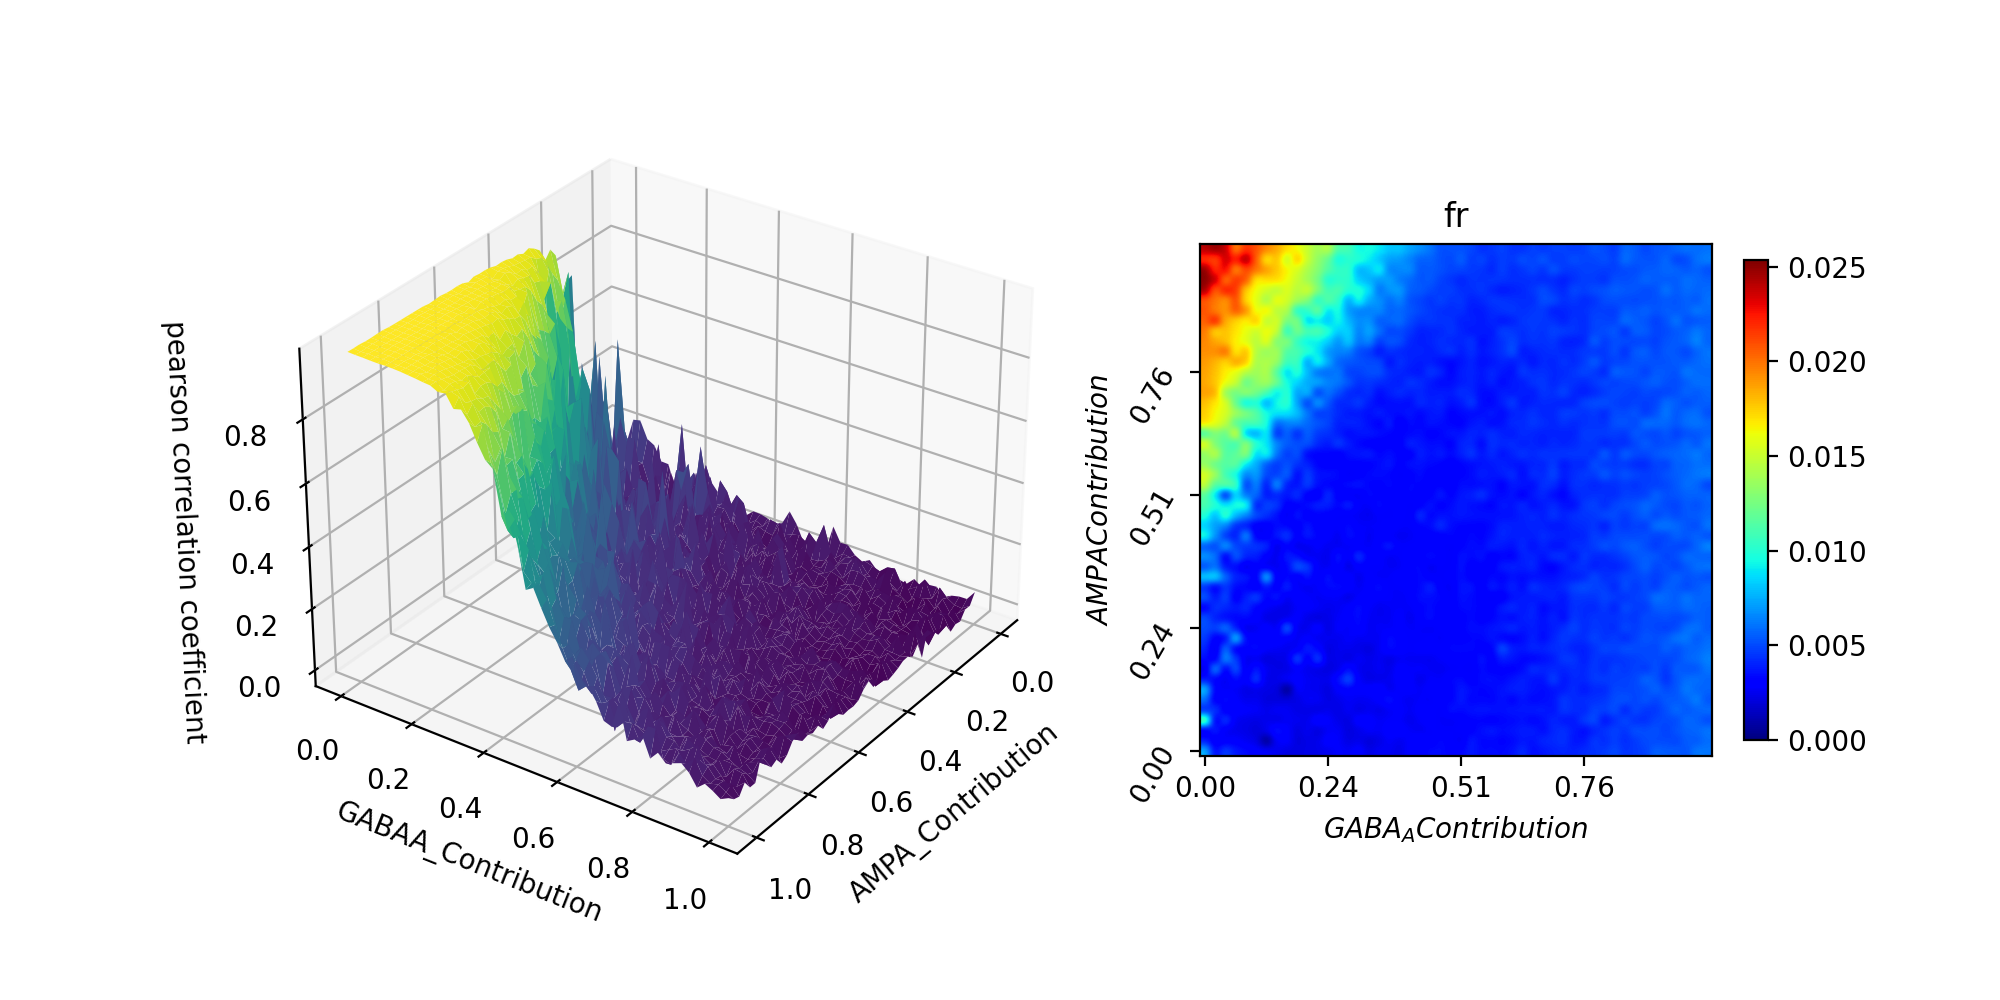
\includegraphics[width=0.85\linewidth]{fig/degree_300}
	\end{figure}
\end{frame}

\begin{frame}{Dependence on connection density}
	grid search on network of 2000 neurons with 500 in-connections.
	\begin{figure}[htbp]
		\centering
		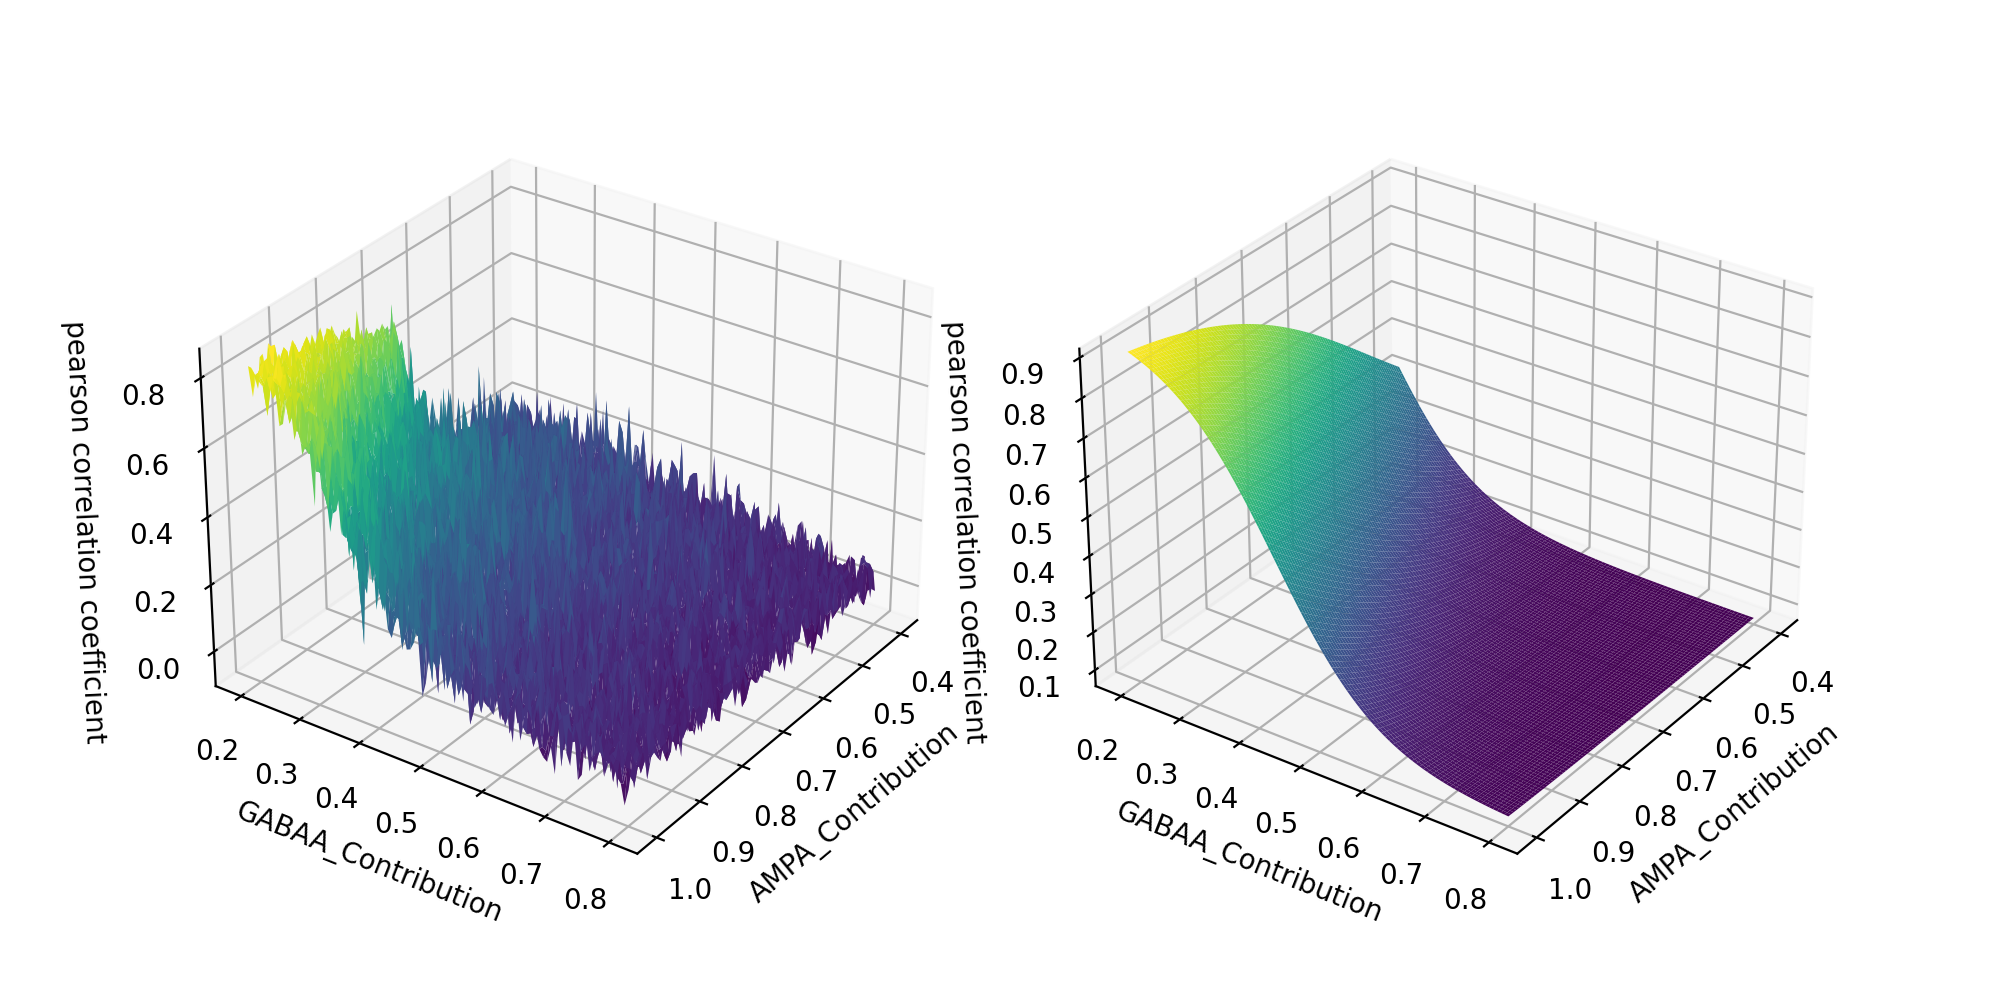
\includegraphics[width=0.85\linewidth]{fig/degree_influence_3d}
	\end{figure}
	As we can see, the plane is much more smooth than its in degree=$ 100 $ and the one-dimensional linear submanifold disappears.
\end{frame}

\begin{frame}{Dependence on connection density}
	If all case fit to function $ s\cdot tanh(ax+by+c) + t $. we can find that its slope is smaller with the degree increasing.
	\begin{figure}[htbp]
		\centering
		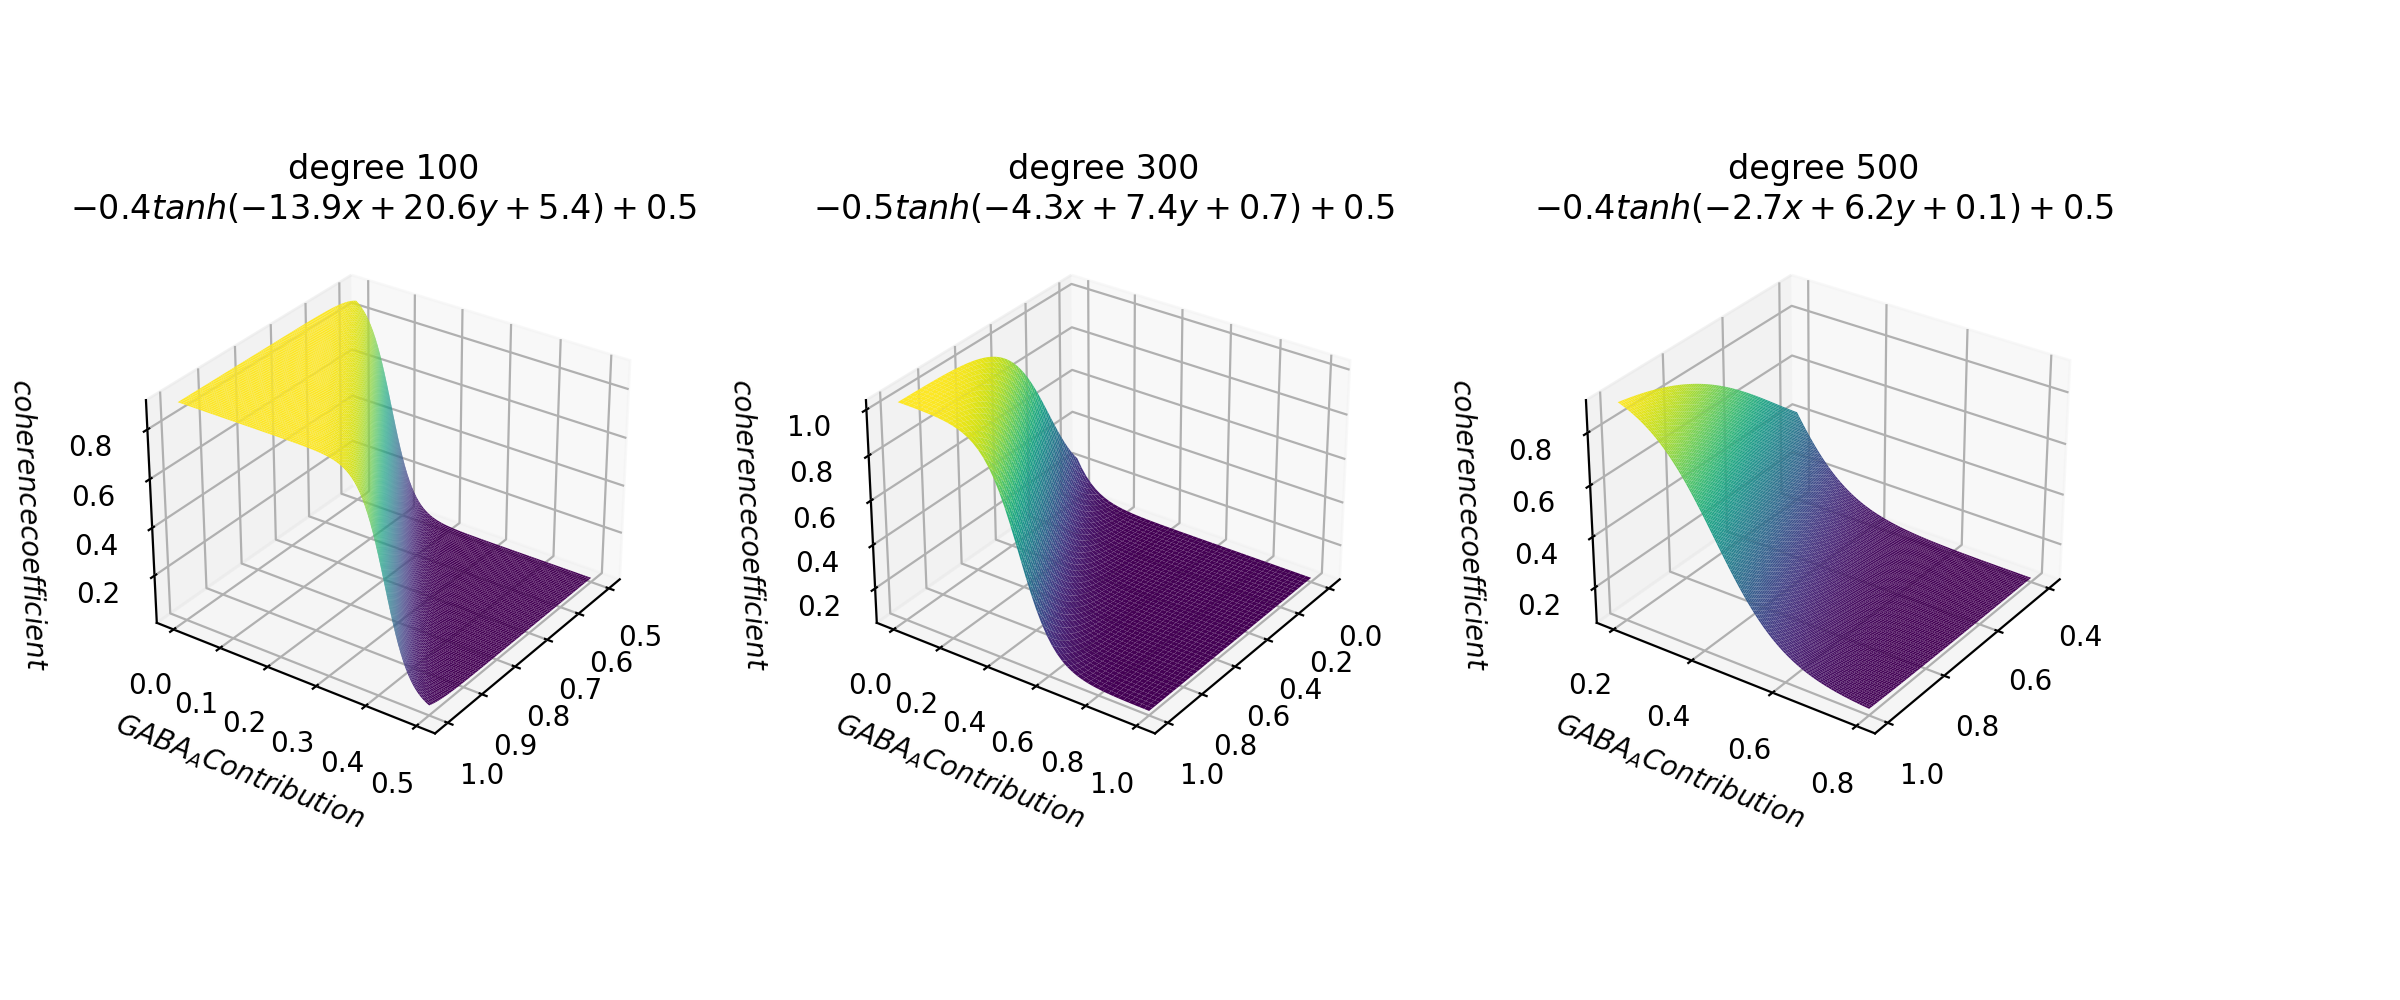
\includegraphics[width=0.85\linewidth]{fig/fit_surface}
	\end{figure}
	
\end{frame}


\subsection{Basic Ideas for Proofs/Implementation}

\begin{frame}{Synaptic drive}
	The full model:
		\begin{equation*}
		\begin{aligned}
			&C_{j} \dot{V_{j}}  = - \sum_{A}g_{L, A}^{j}(V_{j} - E_{A}) \\
			&g_{A}^{j}=c_{A}\sum_{m} \sum_{k|t_{m}^{k}<t}\int_{-\infty}^{t}dt^{\prime}a_{\tau_{decay}}\left(t - t^{\prime}\right) \delta(t^{\prime}-t_{m}^{k}), 
		\end{aligned}
		\end{equation*}
	where $ A= AMPA, NMDA, GABA_{A}, GABA_{B} $.
	\par 
	Herein, only the single neuron properties will be considered. We aim to explore the influence of  restricted parameter $ c_{A} $ to the synaptic drive and membrane response.

\end{frame}

\begin{frame}{The diffusion approximation}
	The number of pulses that arrive within the timescales$ \tau_{A} $ will be approximately gaussian distributed. Thus, we can constitute this Ornstein-Uhlenbeck process.
		\begin{equation}
		\tau_{A} \frac{d g_{A}}{d t} \simeq g_{A 0}-g_{A}+\sqrt{2} \sigma_{A} \xi_{A}(t)
	\end{equation}
	where the gaussian white noise $ \xi_{A} $ has a zero mean and relatively independent.
	\begin{equation}
		\left\langle\xi_{A}(t)\right\rangle=0 \quad\left\langle\xi_{A}(t) \xi_{A}\left(t^{\prime}\right)\right\rangle=\tau_{A} \delta\left(t-t^{\prime}\right)
	\end{equation}
	The average conductance $ g_{A, 0} $ and the standard deviation $ \sigma_{A} $ are related to the variables $ c_{A}, \tau_{A} $ and $ \mathcal{R} $ through
	\begin{equation}
		g_{A 0}=c_{A} \tau_{A} \mathcal{R}_{A}, \quad \sigma_{A}=c_{A}  \sqrt{\frac{\tau_{A}\mathcal{R}_{A}}{2}}
	\end{equation}
\end{frame}

\begin{frame}{The diffusion approximation}
	 we sole the above OU equation, then derive:
	 \begin{equation}
	 	g_{A}(t) = g_{A}(0)e^{-t/\tau_{A}} + g_{A 0} \left( 1 - e^{-t/\tau_{A}}\right) + \sqrt{2} \sigma_{e} \int_{0}^{t} \dfrac{1}{\tau_{A}} e^{-(t - s) / \tau_{A}} dB_{s}, 
	 \end{equation}
 	and 
	 \begin{equation}
	 	g_{A F}(t) \equiv g_{A}(t)-g_{A 0} \simeq \sqrt{2} \sigma_{A} \int_{0}^{t} \dfrac{1}{\tau_{A}} e^{-(t - s) / \tau_{A}} dB_{s}
	 \end{equation}
 	\par 
 	\begin{equation}
 		g_{A F}(t) \sim \mathcal{N}\left(0, 2 \sigma_{A}^{2} \int_{0}^{t} (\dfrac{1}{\tau_{A}}e^{-(t - s) / \tau_{A}})^{2} dt\right) (\text{Ito isometry}) ,
 	\end{equation}
 	if $ t \rightarrow \infty $, 
 	\begin{equation}
 		p_{D}\left(g_{A}\right)=\frac{1}{\sqrt{2 \pi \sigma_{A}^{2}}} \exp \left(-\frac{\left(g_{A}-g_{A 0}\right)^{2}}{2 \sigma_{A}^{2}}\right)
 	\end{equation}
 	
\end{frame}
\begin{frame}{The diffusion approximation}
	The criterion for validity of the approximation is $ \sigma_{A} / g_{A 0} << 1$ .
	\par 
	If we thake consideration of the eq(\ref{eq:param_restriction}) and we can derive the total conductance drive. Thus, using excitation as an example,
	\begin{equation*}
		\frac{d g_{e}}{d t} \simeq \dfrac{g_{0}^{(1)}}{\tau_{1}} + \dfrac{g_{0}^{(2)}}{\tau_{2}} - (\dfrac{\tau_{1}+\tau_{2}}{\tau_{1}\tau_{2}})g_{e}+\sqrt{2} (\dfrac{\tau_{1}\sigma_{1}+\tau_{2}\sigma_{1}}{\tau_{1}\tau_{2}}) \xi_{e}(t) , 
	\end{equation*}
	similarly, we can conclude that the excitatory conducatance obey the gaussian disritbuion.
\end{frame}

\begin{frame}{Membrane response}
	By separating the synaptic conductances into components $ g_{0}^{(i)}, i=1,2,3,4 $, and fluctuating components $ g_{F}^{(i)},i=1, 2, 3, 4 $.
	\begin{equation}
		C \frac{d V}{d t}=-g_{0}\left(V-E_{0}\right)-\sum_{i=1}^{4}g_{F}^{(i)}\left(V-E_{i}\right)
	\end{equation}
	where
	\begin{equation}
		g_{0}=g_{L}+\sum g_{0}^{(i)} \quad \text { and } \quad E_{0}=\frac{1}{g_{0}}\left(g_{L} E_{L}+\sum g_{0}^{(i)} E_{i}\right)
	\end{equation}
	effective membrane time constant: $ \tau_{0} = C /g_{0} $
\end{frame}
\begin{frame}{Membrane response}
	the voltage-dependent component of the drive can be expanded around the equilibrium potential $ E_{0} $
	\begin{equation}
		g_{F}^{i}\left(V-E_{i}\right)=g_{F}^{i}\left(E_{0}-E_{i}\right)+g_{F}^{i}\left(V-E_{i}\right)
	\end{equation}
	\par
	If we drope the multiplicative noise term, that is
	\begin{equation}
		\label{eq: constant_approximation}
		\left\{
		\begin{aligned}	
		&C \frac{d V}{d t} \simeq-g_{0}\left(V-E_{0}\right)+\sum g_{F}^{i}\left(E_{i}-E_{0}\right) \\
		&\tau_{i} \frac{d g_{F}^{o}}{d t} \simeq g_{F}^{i}+\sqrt{2} \sigma_{i} \xi_{i}(t)
	\end{aligned}
	\right .
	\end{equation}
	where, $ \xi_{1} $ and $ \xi_{2} $ is totally correlated, $ \xi_{3} $ and $ \xi_{4} $ is totally correlated.
\end{frame}
\begin{frame}{Membrane response}
	Then we can rewrite the eq\ref{eq: constant_approximation} as:
	\begin{equation}
		\dfrac{dV}{dt} \simeq -\dfrac{1}{\tau_{0}}\left(V - E_{0}\right) + I_{F}
	\end{equation}
	and we have
	\begin{equation}
		\begin{aligned}
			I_{F}(t)  &= V(t)-E_{0} \\
			 &\simeq \sum \sqrt{2}\left(\frac{\sigma_{i}}{g_{0}}\right) \frac{\left(E_{i}-E_{0}\right)}{\left(\tau_{i}-\tau_{0}\right)} \int_{0}^{\infty} d s\left(e^{-s / \tau_{i}}-e^{-s / \tau_{0}}\right) \xi_{i}(t-s)
		\end{aligned}
	\end{equation}
\end{frame}

\begin{frame}{Membrane response}
	The distribution predicted for the voltage is the gaussian
	\begin{equation}
		p_{0}(V)=\frac{1}{\sqrt{2 \pi \sigma_{V}^{2}}} \exp \left(-\frac{\left(V-E_{0}\right)^{2}}{2 \sigma_{V}^{2}}\right)
	\end{equation}
	where, for the case where there are no correlations between excitation and
	inhibition, the variance is 
	\begin{equation*}
	\begin{aligned}
		\sigma_{V}^{2}&=\sum_{i=1}^{4}\left(\frac{\sigma_{i}}{g_{0}}\right)^{2}\left(E_{i}-E_{0}\right)^{2} \frac{\tau_{i}}{\left(\tau_{i}+\tau_{0}\right)} \\
		&+ 2\left(\frac{\sigma_{1} \sigma_{2}}{g_{0}^{2}}\right)\left(E_{1}-E_{0}\right)\left(E_{2}-E_{0}\right) \frac{\sqrt{\tau_{1} \tau_{2}}\left(2 \tau_{1} \tau_{2}+\tau_{1} \tau_{0}+\tau_{2} \tau_{0}\right)}{\left(\tau_{1}+\tau_{2}\right)\left(\tau_{1}+\tau_{0}\right)\left(\tau_{2}+\tau_{0}\right)} \\
		&+ 2\left(\frac{\sigma_{3} \sigma_{4}}{g_{0}^{2}}\right)\left(E_{3}-E_{0}\right)\left(E_{4}-E_{0}\right) \frac{\sqrt{\tau_{3} \tau_{4}}\left(2 \tau_{3} \tau_{4}+\tau_{3} \tau_{0}+\tau_{4} \tau_{0}\right)}{\left(\tau_{3}+\tau_{4}\right)\left(\tau_{3}+\tau_{0}\right)\left(\tau_{4}+\tau_{0}\right)}
	\end{aligned}
	\end{equation*}
\end{frame}

\begin{frame}{Membrane response}
	Increasing $ GABA_{A} $ modifies the equilibrium value $ E_{0} $, the drift force and the input noise.
	\begin{figure}[htbp]
		\centering
		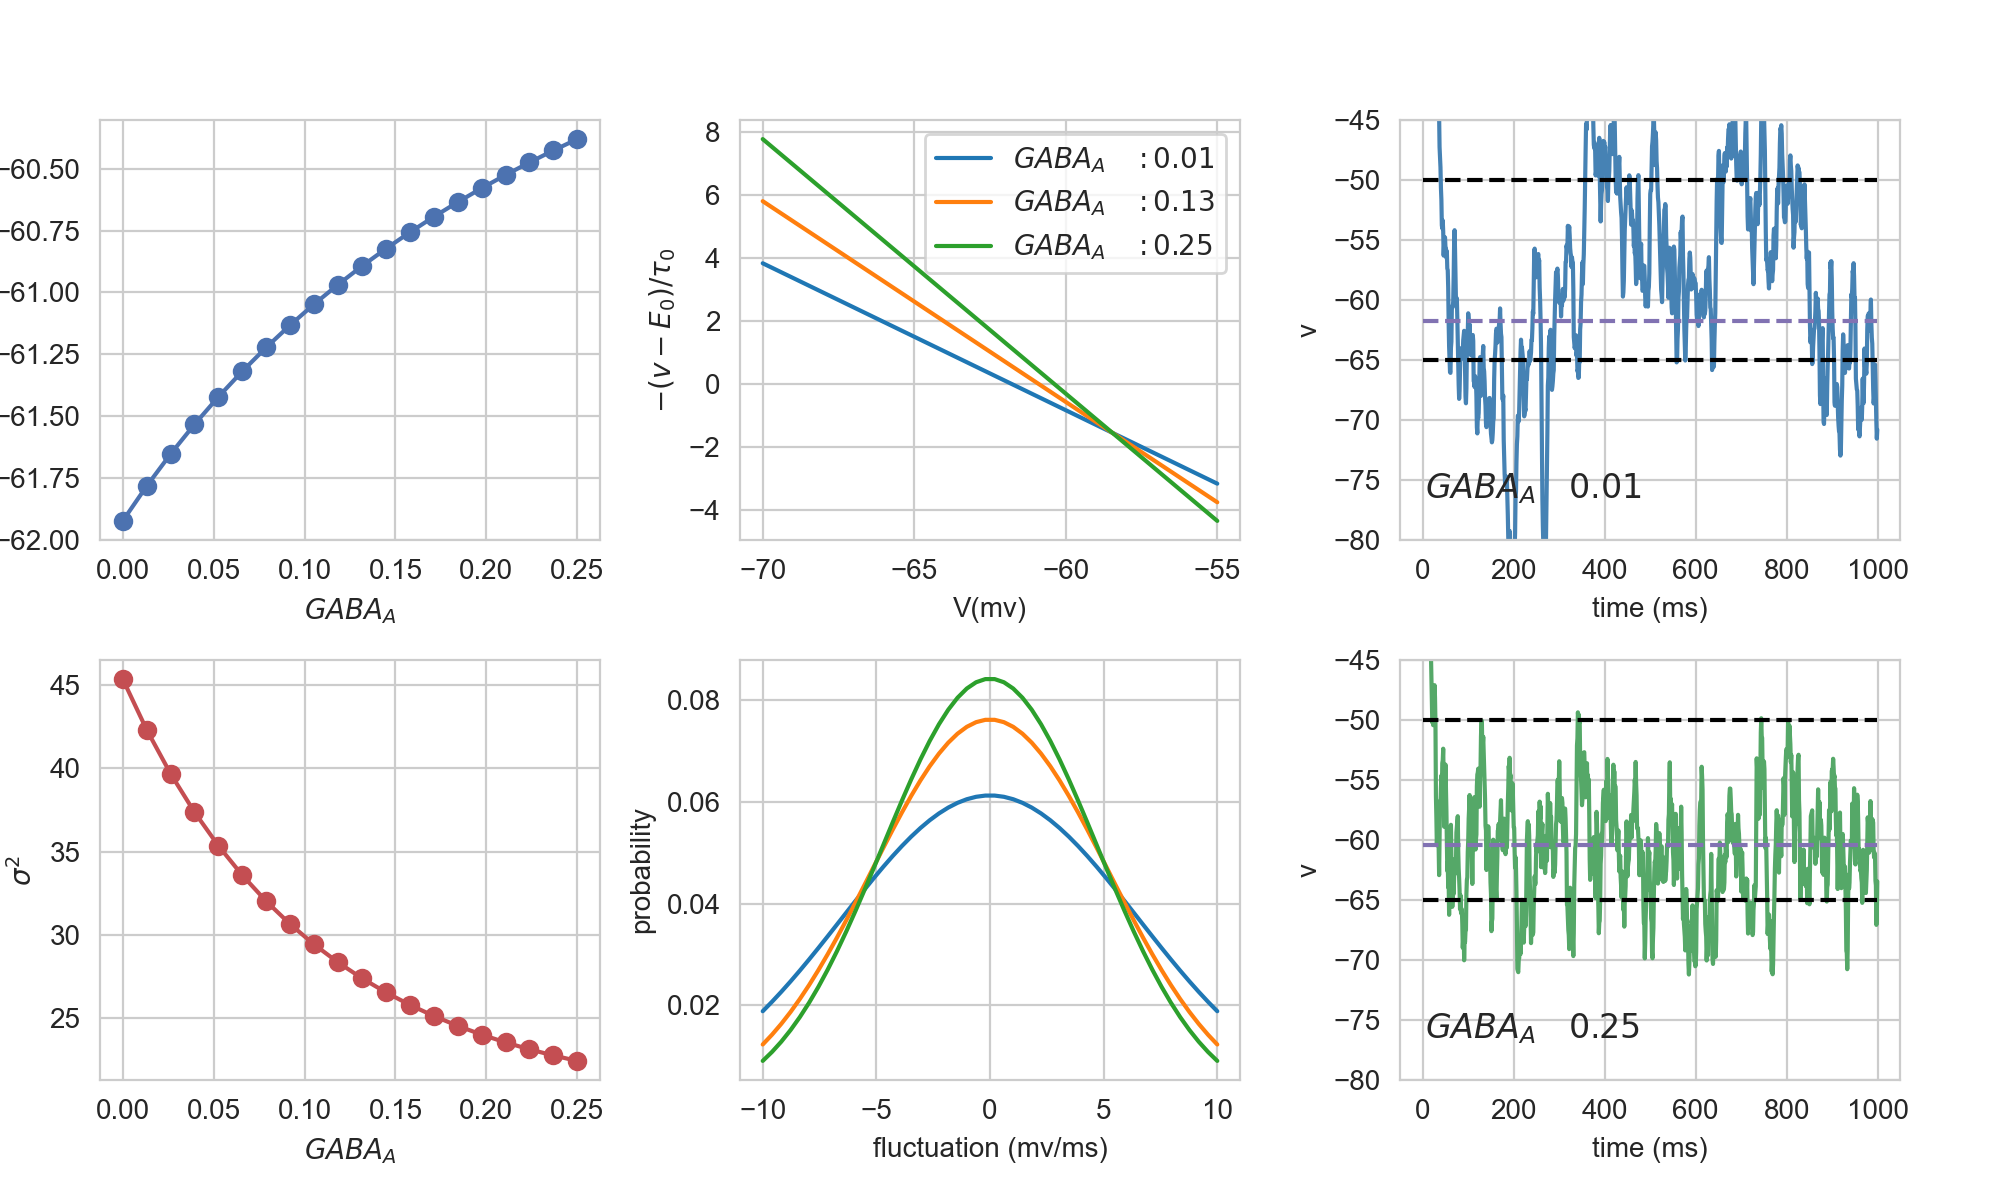
\includegraphics[width=0.75\linewidth]{fig/diffusion_theorem}
		\caption{Effects of GABAA on the friing behavior of isolated conductance-based neuron}
	\end{figure}
\end{frame}
\begin{frame}{input-output correlation}
		\begin{figure}[htbp]
		\centering
		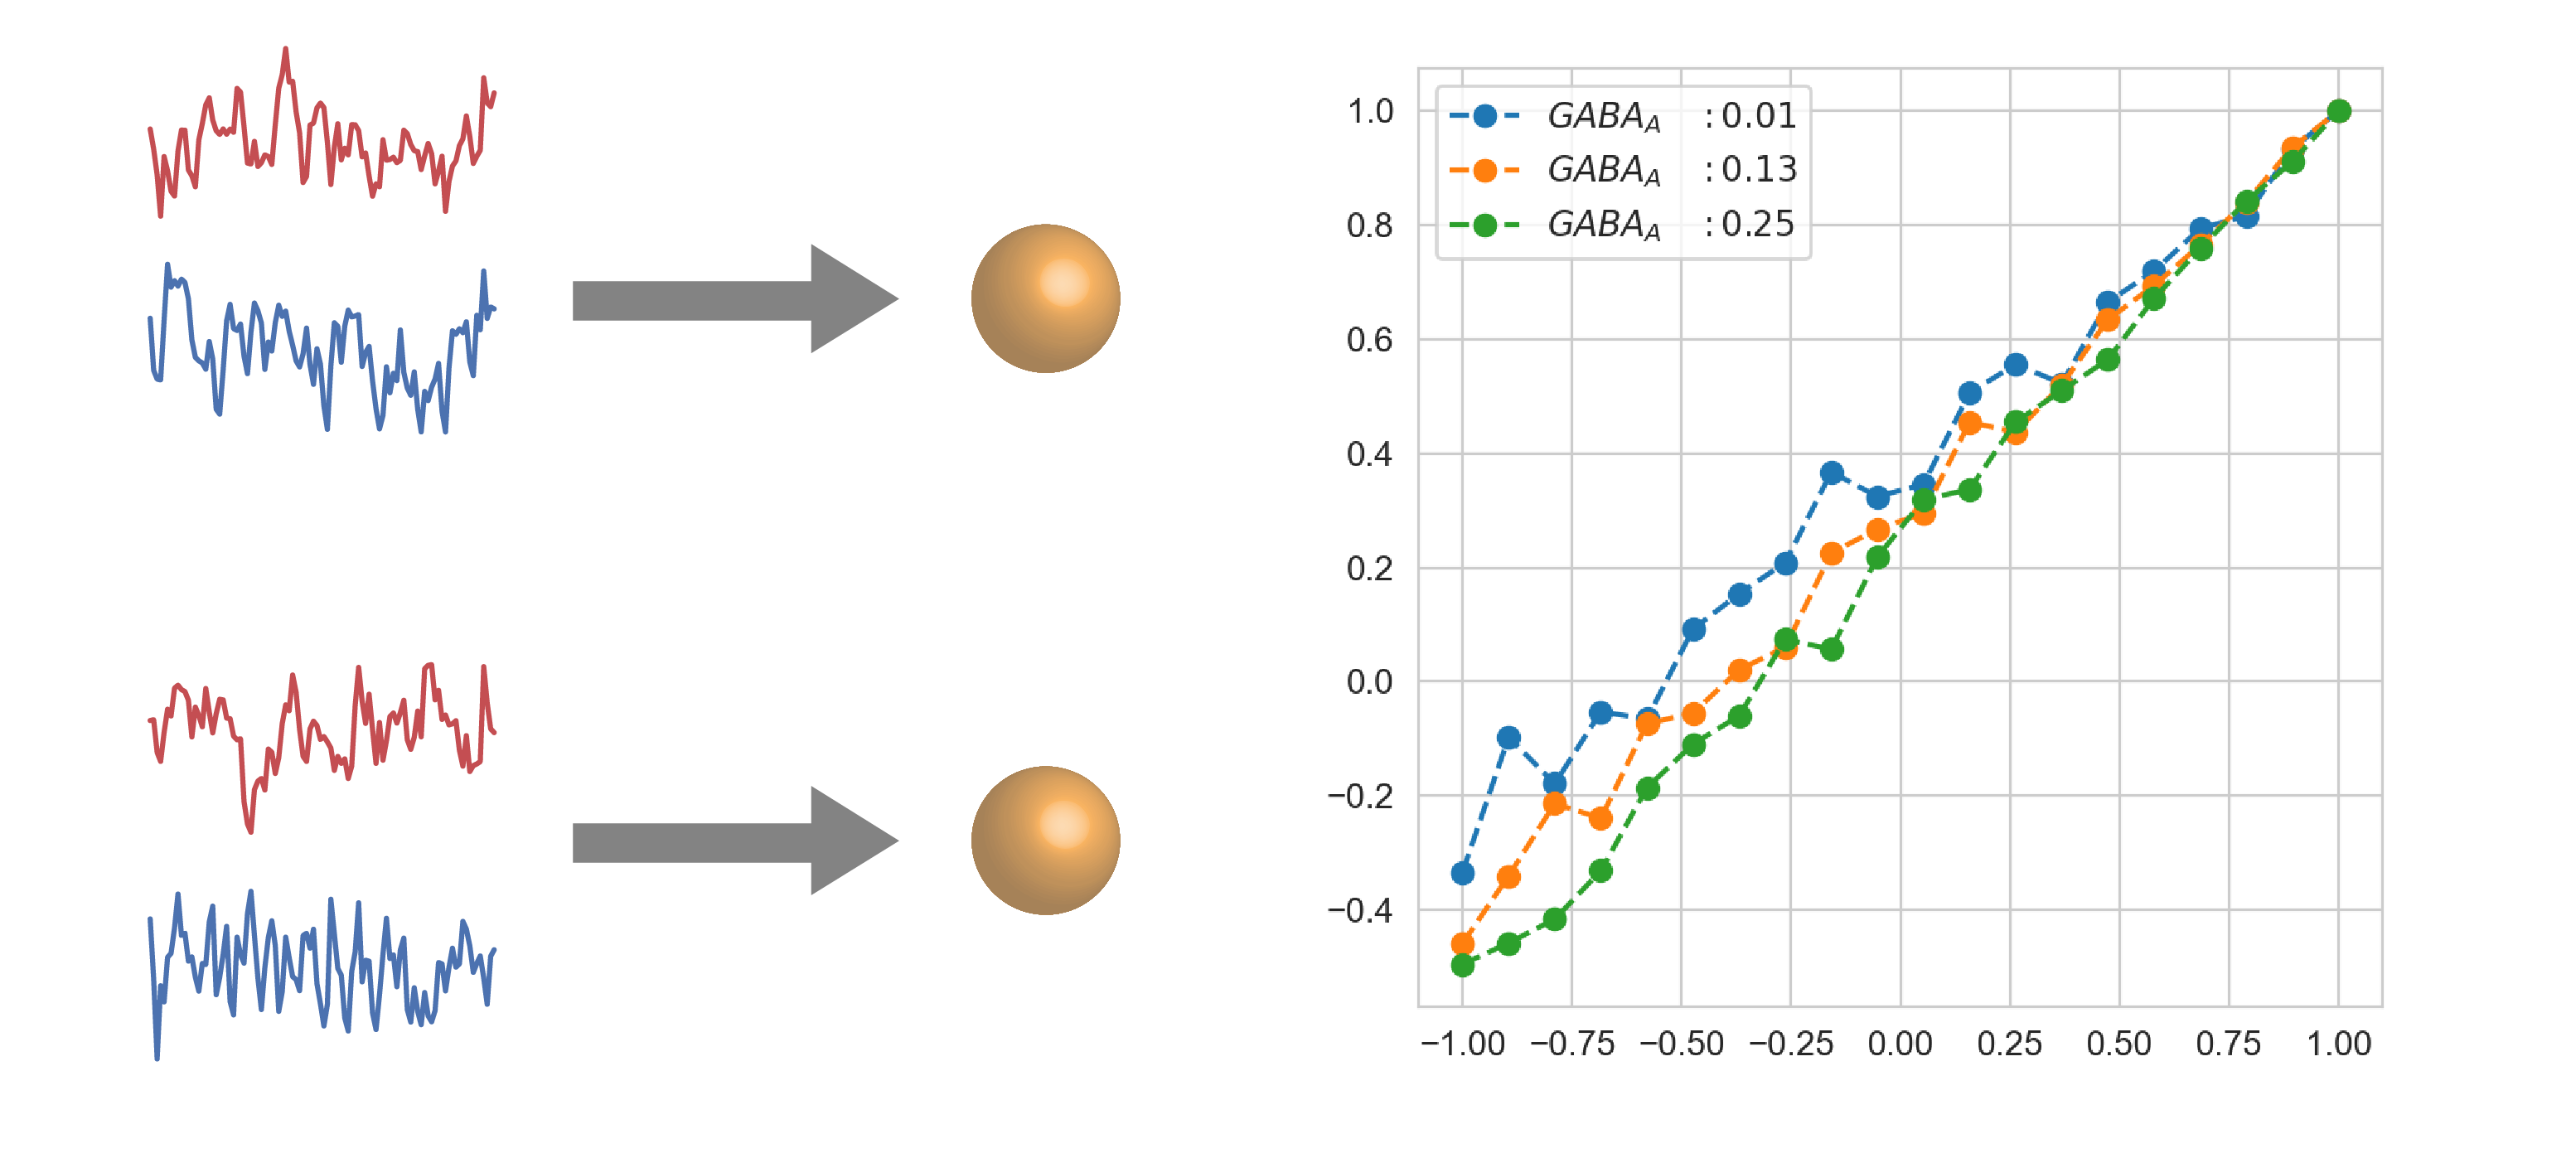
\includegraphics[width=0.85\linewidth]{fig/correlate}
		\caption{The relationship between the input and output correlation coefficients for an LIF neuron}
	\end{figure}
\end{frame}

\section*{Summary}

\begin{frame}{Summary}

  % Keep the summary *very short*.
  \begin{itemize}
  \item
    The \alert{first main message} of your talk in one or two lines.
  \item
    The \alert{second main message} of your talk in one or two lines.
  \item
    Perhaps a \alert{third message}, but not more than that.
  \end{itemize}
  
  % The following outlook is optional.
  \vskip0pt plus.5fill
  \begin{itemize}
  \item
    Outlook
    \begin{itemize}
    \item
      Something you haven't solved.
    \item
      Something else you haven't solved.
    \end{itemize}
  \end{itemize}
\end{frame}



% All of the following is optional and typically not needed. 
\appendix
\section<presentation>*{\appendixname}
\subsection<presentation>*{For Further Reading}

\begin{frame}[allowframebreaks]
  \frametitle<presentation>{For Further Reading}
    
  \begin{thebibliography}{10}
    
  \beamertemplatebookbibitems
  % Start with overview books.

  \bibitem{Author1990}
    A.~Author.
    \newblock {\em Handbook of Everything}.
    \newblock Some Press, 1990.
 
    
  \beamertemplatearticlebibitems
  % Followed by interesting articles. Keep the list short. 

  \bibitem{Someone2000}
    S.~Someone.
    \newblock On this and that.
    \newblock {\em Journal of This and That}, 2(1):50--100,
    2000.
  \end{thebibliography}
\end{frame}

\end{document}


